%----------
%	CONFIGURACIÓN DEL DOCUMENTO
%----------

% Definimos las características del documento y añadimos una serie de paquetes (\usepackage{package}) que agregan funcionalidades a LaTeX.

\documentclass[12pt]{report} %fuente a 12pt

% MÁRGENES: 2,5 cm sup. e inf.; 3 cm izdo. y dcho.
\usepackage[
a4paper,
vmargin=2.5cm,
hmargin=3cm
]{geometry}

% INTERLINEADO: Estrecho (6 ptos./interlineado 1,15) o Moderado (6 ptos./interlineado 1,5)
\renewcommand{\baselinestretch}{1.15}
\parskip=6pt

% DEFINICIÓN DE COLORES para portada y listados de código
\usepackage[table]{xcolor}
\definecolor{azulUC3M}{RGB}{0,0,102}
\definecolor{gray97}{gray}{.97}
\definecolor{gray75}{gray}{.75}
\definecolor{gray45}{gray}{.45}

% Soporte para GENERAR PDF/A --es importante de cara a su inclusión en e-Archivo porque es el formato óptimo de preservación y a la generación de metadatos, tal y como se describe en http://uc3m.libguides.com/ld.php?content_id=31389625. En la carpeta incluímos el archivo plantilla_tfg_2017.xmpdata en el que puedes incluir los metadatos que se incorporarán al archivo PDF cuando lo compiles. Ese archivo debe llamarse igual que tu archivo .tex. Puedes ver un ejemplo en esta misma carpeta.
\usepackage[a-1b]{pdfx}

% ENLACES
\usepackage{hyperref}
\hypersetup{colorlinks=true,
	linkcolor=black, % enlaces a partes del documento (p.e. índice) en color negro
	urlcolor=blue} % enlaces a recursos fuera del documento en azul

% EXPRESIONES MATEMATICAS
\usepackage{amsmath,amssymb,amsfonts,amsthm}

\usepackage{txfonts} 
\usepackage[T1]{fontenc}
\usepackage[utf8]{inputenc}

\usepackage[spanish, es-tabla]{babel} 
\usepackage[babel, spanish=spanish]{csquotes}
\usepackage{etoolbox}
\AtBeginEnvironment{quote}{\small}

% diseño de PIE DE PÁGINA
\usepackage{fancyhdr}
\pagestyle{fancy}
\fancyhf{}
\renewcommand{\headrulewidth}{0pt}
\rfoot{\thepage}
\fancypagestyle{plain}{\pagestyle{fancy}}

% DISEÑO DE LOS TÍTULOS de las partes del trabajo (capítulos y epígrafes o subcapítulos)
\usepackage{titlesec}
\usepackage{titletoc}
\titleformat{\chapter}[block]
{\large\bfseries\filcenter}
{\thechapter.}
{5pt}
{\MakeUppercase}
{}
\titlespacing{\chapter}{0pt}{0pt}{*3}
\titlecontents{chapter}
[0pt]                                               
{}
{\contentsmargin{0pt}\thecontentslabel.\enspace\uppercase}
{\contentsmargin{0pt}\uppercase}                        
{\titlerule*[.7pc]{.}\contentspage}                 

\titleformat{\section}
{\bfseries}
{\thesection.}
{5pt}
{}
\titlecontents{section}
[5pt]                                               
{}
{\contentsmargin{0pt}\thecontentslabel.\enspace}
{\contentsmargin{0pt}}
{\titlerule*[.7pc]{.}\contentspage}

\titleformat{\subsection}
{\normalsize\bfseries}
{\thesubsection.}
{5pt}
{}
\titlecontents{subsection}
[10pt]                                               
{}
{\contentsmargin{0pt}                          
	\thecontentslabel.\enspace}
{\contentsmargin{0pt}}                        
{\titlerule*[.7pc]{.}\contentspage}  


% DISEÑO DE TABLAS. Puedes elegir entre el estilo para ingeniería o para ciencias sociales y humanidades. Por defecto, está activado el estilo de ingeniería. Si deseas utilizar el otro, comenta las líneas del diseño de ingeniería y descomenta las del diseño de ciencias sociales y humanidades
\usepackage{multirow} % permite combinar celdas 
\usepackage{caption} % para personalizar el título de tablas y figuras
\usepackage{floatrow} % utilizamos este paquete y sus macros \ttabbox y \ffigbox para alinear los nombres de tablas y figuras de acuerdo con el estilo definido. Para su uso ver archivo de ejemplo 
\usepackage{array} % con este paquete podemos definir en la siguiente línea un nuevo tipo de columna para tablas: ancho personalizado y contenido centrado
\newcolumntype{P}[1]{>{\centering\arraybackslash}p{#1}}
\DeclareCaptionFormat{upper}{#1#2\uppercase{#3}\par}

% Diseño de tabla para ingeniería
\captionsetup[table]{
	format=upper,
	name=TABLA,
	justification=centering,
	labelsep=period,
	width=.75\linewidth,
	labelfont=small,
	font=small,
}

%Diseño de tabla para ciencias sociales y humanidades
%\captionsetup[table]{
%	justification=raggedright,
%	labelsep=period,
%	labelfont=small,
%	singlelinecheck=false,
%	font={small,bf}
%}


% DISEÑO DE FIGURAS. Puedes elegir entre el estilo para ingeniería o para ciencias sociales y humanidades. Por defecto, está activado el estilo de ingeniería. Si deseas utilizar el otro, comenta las líneas del diseño de ingeniería y descomenta las del diseño de ciencias sociales y humanidades
\usepackage{graphicx}
\graphicspath{{res/}} %ruta a la carpeta de imágenes

\usepackage{afterpage}
% Diseño de figuras para ingeniería
\captionsetup[figure]{
	format=hang,
	name=Fig.,
	singlelinecheck=off,
	labelsep=period,
	labelfont=small,
	font=small		
}


% NOTAS A PIE DE PÁGINA
\usepackage{chngcntr} %para numeración contínua de las notas al pie
\counterwithout{footnote}{chapter}

% LISTADOS DE CÓDIGO
% soporte y estilo para listados de código. Más información en https://es.wikibooks.org/wiki/Manual_de_LaTeX/Listados_de_código/Listados_con_listings
\usepackage{listings}

% definimos un estilo de listings
\lstdefinestyle{estilo}{ frame=Ltb,
	framerule=0pt,
	aboveskip=0.5cm,
	framextopmargin=3pt,
	framexbottommargin=3pt,
	framexleftmargin=0.4cm,
	framesep=0pt,
	rulesep=.4pt,
	backgroundcolor=\color{gray97},
	rulesepcolor=\color{black},
	%
	basicstyle=\ttfamily\footnotesize,
	keywordstyle=\bfseries,
	stringstyle=\ttfamily,
	showstringspaces = false,
	commentstyle=\color{gray45},     
	%
	numbers=left,
	numbersep=15pt,
	numberstyle=\tiny,
	numberfirstline = false,
	breaklines=true,
	xleftmargin=\parindent
}

\captionsetup[lstlisting]{font=small, labelsep=period}
% fijamos el estilo a utilizar 
\lstset{style=estilo}
\renewcommand{\lstlistingname}{\uppercase{Código}}


%BIBLIOGRAFÍA - PUEDES ELEGIR ENTRE ESTILO IEEE O APA. POR DEFECTO ESTÁ CONFIGURADO IEEE. SI DESEAS USAR APA, COMENTA LAS LÍNEA DE IEEE Y DESCOMENTA LAS DE APA. Si haces cambios en la configuración de la bibliografía y no obtienes los resultados esperados, es recomendable limpiar los archivos auxiliares y volver a compilar en este orden: COMPILAR-BIBLIOGRAFIA-COMPILAR

% Tienes más información sobre cómo generar bibliografía y CONFIGURAR TU EDITOR DE TEXTO para compilar con biber en http://tex.stackexchange.com/questions/154751/xx-with-biber-configuring-my-editor-to-avoid-undefined-citations , https://www.overleaf.com/learn/latex/Bibliography_management_in_LaTeX y en http://www.ctan.org/tex-archive/macros/latex/exptl/biblatex-contrib
% También te recomendamos consultar la guía temática de la Biblioteca sobre citas bibliográficas: http://uc3m.libguides.com/guias_tematicas/citas_bibliograficas/inicio

% CONFIGURACIÓN PARA LA BIBLIOGRAFÍA IEEE
\usepackage[backend=biber, style=ieee, isbn=false,sortcites, maxbibnames=5, minbibnames=1]{biblatex} % Configuración para el estilo de citas de IEEE, recomendado para el área de ingeniería. "maxbibnames" indica que a partir de 5 autores trunque la lista en el primero (minbibnames) y añada "et al." tal y como se utiliza en el estilo IEEE.

% Añadimos las siguientes indicaciones para mejorar la adaptación de los estilos en español
\DefineBibliographyStrings{spanish}{%
	andothers = {et\addabbrvspace al\adddotspace}
}
\DefineBibliographyStrings{spanish}{
	url = {\adddotspace[En línea]\adddotspace Disponible en:}
}
\DefineBibliographyStrings{spanish}{
	urlseen = {Acceso:}
}
\DefineBibliographyStrings{spanish}{
	pages = {pp\adddotspace},
	page = {p.\adddotspace}
}


\addbibresource{bib/bibliography.bib} % llama al archivo bibliografia.bib en el que debería estar la bibliografía utilizada

% my settings
\linespread{1.5}
\usepackage{float}
\usepackage[bottom]{footmisc}
\usepackage{enumitem}
\newcommand{\sigmadelta}{$\Sigma\Delta\; $}
\usepackage{microtype}
\usepackage{multicol}
\usepackage{listings}


%-------------
%	DOCUMENTO
%-------------

\begin{document}
\pagenumbering{roman} % Se utilizan cifras romanas en la numeración de las páginas previas al cuerpo del trabajo

%----------
%	PORTADA
%----------	
\begin{titlepage}

	\begin{sffamily}
	\color{azulUC3M}
	\begin{center}
		\begin{figure}[H] %incluimos el logotipo de la Universidad
			\makebox[\textwidth][c]{
\includegraphics[width=16cm]{res/Portada_Logo.png}}
		\end{figure}
		\vspace{2.5cm}
		\begin{Large}
			Grado en Ingeniería en Tecnologías Industriales		
			2019-2020
			\vspace{2cm}		
			\textsl{Trabajo de Fin de Grado}
			\bigskip
			
		\end{Large}
		 	{\Huge LINEALIZACIÓN DE OSCILADOR EN ANILLO CONTROLADO POR TENSIÓN MEDIANTE CAPACIDADES CONMUTADAS}\\
		 	\vspace*{0.5cm}
	 		\rule{10.5cm}{0.1mm}\\
			\vspace*{0.9cm}
			{\LARGE Roberto Uceda Gómez}\\ 
			\vspace*{1cm}
		\begin{Large}
			Tutor:
			Eric Gutiérrez Fernández \\
			Leganés, %TODO: fecha \\
		\end{Large}
	\end{center}
	\vfill
	\color{black}
	% si nuestro trabajo se va a publicar con una licencia Creative Commons, incluir estas líneas. Es la opción recomendada.
	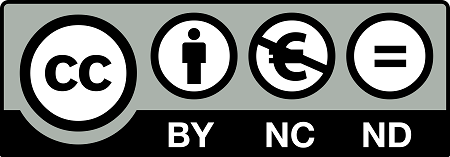
\includegraphics[width=4.2cm]{res/creativecommons.png}\\ %incluimos el logotipo de creativecommons
	Esta obra se encuentra sujeta a la licencia Creative Commons\\ \textbf{Reconocimiento - No Comercial - Sin Obra Derivada}
	\end{sffamily}
\end{titlepage}

\newpage %página en blanco o de cortesía
\thispagestyle{empty}
\mbox{}

%----------
%	RESUMEN Y PALABRAS CLAVE
%----------	
\renewcommand\abstractname{\large\bfseries\filcenter\uppercase{Resumen}}
\begin{abstract}
\thispagestyle{plain}
\setcounter{page}{3}
	
	% ESCRIBIR EL RESUMEN AQUÍ
	En este trabajo se desarrolla un estudio cuyo objetivo es encontrar una manera de linealizar el comportamiento de una nueva arquitectura de ADC basado en VCO, sin necesidad del uso de amplificador operacional, como se ha hecho hasta ahora.
	
	\textbf{Palabras clave: ADC-VCO, Oscilador en anillo, Conversión Analógico-Digital, CMOS}
	% Escribir las palabras clave aquí
	
	%TODO
	\vfill
\end{abstract}
	\newpage % página en blanco o de cortesía
	\thispagestyle{empty}
	\mbox{}


%----------
%	DEDICATORIA
%----------	
\chapter*{Dedicatoria}

\setcounter{page}{5}
	
	%TODO
		
	\vfill
	
	\newpage % página en blanco o de cortesía
	\thispagestyle{empty}
	\mbox{}
	

%----------
%	ÍNDICES
%----------	

%--
% Índice general
%-
\tableofcontents
\thispagestyle{fancy}


%--
% Índice de figuras. Si no se incluyen, comenta las líneas siguientes
%-
\listoffigures
\thispagestyle{fancy}


%--
% Índice de tablas. Si no se incluyen, comenta las líneas siguientes
%-
\listoftables
\thispagestyle{fancy}


%--
% Lista de abreviaturas. Si no se incluyen, comenta las líneas siguientes
%-
\newpage
\begin{table}[h!]
	\setlength{\arrayrulewidth}{0mm}
	\begin{center}
		\caption{Lista de abreviaturas}
		\label{tab:table1}
		\begin{tabular}{>{\bf}p{4cm}|p{10cm}}
			ADC & Analog to Digital Converter, Convertidor Analógico-Digital \\
			CMOS & Complimentary Metal-Oxide Semiconductor \\
			MOSFET & Metal Oxide Semiconductor Field Effect Transistor, también llamados transistores MOS \\
		\end{tabular}
	\end{center}
\end{table}

\newpage % página en blanco o de cortesía
\thispagestyle{empty}
\mbox{}

%----------
%	TRABAJO
%----------	
\clearpage
\pagenumbering{arabic} % numeración con múmeros arábigos para el resto de la publicación	

\chapter{Introducción}

	Los ADC\footnote{Analog to Digital Converter. En español, Convertidor Analógico a Digital} son onmipresentes en nuestro día a día. Sin ellos, no sería posible realizar una llamada con un teléfono móvil, o disfrutar de un sistema de climatización en nuestro hogar, o utilizar el control de crucero en nuestro coche. El objetivo de estos importantes bloques de la electrónica es convertir señales físicas, como ondas electromagnéticas, temperatura ambiente, o la posición de un eje, en señales digitales interpretables por un sistema basado en la electrónica digital. Una vez tenemos estas señales, normalmente compuestas por un flujo de bits, pueden ser procesadas por un microcontrolador para después tomar las decisiones necesarias para conseguir el objetivo deseado, como activar el compresor del aire acondicionado si la temperatura sube de cierto límite preestablecido.
	
	Cada día que pasa aumenta la demanda de aparatos más rápidos, compactos, y eficientes. Por regla general, la miniaturización de la electrónica tiene un impacto positivo en estos criterios. Los transistores son los componentes fundamentales de los circuitos integrados. Estos transistores aumentan su eficiencia energética según disminuye su tamaño, además de permitir mayores frecuencias de operación. Por esto, existe un gran incentivo en la búsqueda de arquitecturas y técnicas de fabricación que permitan transistores más pequeños.
	
	La ley de Moore ayuda a poner un poco de contexto histórico a esta carrera por la disminución de los transistores. Gordon Moore anunció en 1965 una tendencia en la, por aquel entonces emergente, industria de la electrónica: cada dos años se duplicaba la cantidad de componentes presente en un circuito integrado en la misma superficie \cite{moorelaw}. A más componentes, mayor poder de procesamiento, pero también mayor coste de fabricación por la complejidad y delicadeza requerida en los procesos.
	
	\section{Motivación del trabajo}
	
	Debido a las altas velocidades de reloj y los requisitos de consumo y fabricación (espacio ocupado, número de componentes, reducción del tamaño de los transistores), los ADC usados actualmente presentan problemas. Los ADC basados en la arquitectura sigma delta, los más comunes en aplicaciones de bajo ancho de banda y alta resolución (audio, sensores biométricos y de alta precisión), requieren de un integrador. Estos integradores normalmente trabajan en el ámbito analógico, y la gran mayoría usan un amplificador operacional, con gran número de componentes y alto consumo.
	
	Con las tecnologías de fabricación actuales, se consiguen transistores de tamaños diminutos, con buen tiempo de respuesta y bajo consumo en aplicaciones digitales, pero efectos adversos en aplicaciones analógicas.
	%TODO: ERIC: pon algún ejemplo numérico
	Algunos de estos efectos son la degradación de la señal por efectos cuánticos y defectos en la fabricación (el tamaño nominal de un transistor CMOS de tecnología puntera es entre un cuarto y una décima parte la longitud de onda de la luz ultravioleta usada en litografía), altas corrientes parásitas por el bajo tamaño de la puerta del transistor, y limitaciones en la simulación de sistemas por la alta densidad y complejidad en los microchips actuales. Otro efecto negativo que tiene la miniaturización en el diseño de microcircuitos es la falta de escalabilidad de la tensión de corte de los MOSFET. Mientras que la tensión de alimentación baja con el tamaño, la de corte no lo hace en la misma medida, haciendo más difícil el diseño de estructuras de alta ganancia, como los amplificadores operacionales, que requieren de suficiente diferencia entre ambas tensiones.
	
	Además, a pesar de que el consumo individual de los transistores disminuye al reducirse su tamaño, lo hace de manera lineal, mientras que su incremento en número por unidad de superficie crece de manera cuadrática. Esto provoca un gran problema en cuanto a disipación térmica, por eso aumentar el número de componentes en circuitos integrados no es una solución en ciertos casos en que no pueda gestionarse correctamente el calor generado, como en sistemas embebidos y aplicaciones de muy bajo consumo, como dispositivos del IoT\footnote{Internet of Things. En español: Internet de las Cosas}.
	
	Los ADC basados en VCO actuales necesitan una compensación de linealidad mediante circuitería digital, que termina ocupando la mayor parte de la superficie del chip. Este trabajo se centra en la búsqueda de una nueva arquitectura usando un VCO tanto como integrador como cuantificador, que permita ahorrar la necesidad de circuitos de compensación y circuitos analógicos complejos (amplificadores operacionales), manteniendo o mejorando el comportamiento lineal, la resolución, y el ancho de banda de las arquitecturas ya existentes.
	
	\section{Objetivos}
	
	El grueso de este trabajo se encuentra en el plano teórico. El primer paso es realizar un estudio de las arquitecturas de ADC ya existentes, centrándose en aquellas que emplean VCOs. A partir de este estudio, se estudiará la viabilidad de varias ideas de diferentes publicaciones que aún no han sido implementadas. Para esto, se utilizarán herramientas de simulación basadas en SPICE. Una vez probada la efectividad de la arquitectura, la siguiente tarea será montar un circuito con componentes discretos sobre protoboard, medir los parámetros de funcionamiento, y así dejar demostrada la factibilidad de la arquitectura.
	%TODO: consultar Eric

	\section{Marco regulador}
	%TODO: ERIC: Apenas se podría decir algo, pero debes decirlo. Puedes hablar de las aplicaciones del sistema, por ejemplo para un micrófono y de ahí enlazar con la ley de privacidad por grabar con el micrófono la voz de la gente. Llévalo a la aplicación concreta y ahí habla de leyes de privacidad, almacenamiento de datos...
	
	
	\section{Esquema de este documento}
	%TODO por decidir
	

	
	

\chapter{Estado del arte}

	Para entender las arquitecturas de ADC modernas es imprescindible conocer primero los bloques fundamentales sobre los que se asienta la microelectrónica actualmente: los transistores MOSFET\footnote{Metal Oxide Semiconductor Field Effect Transistor}.
	
	\section{Transistores MOS}
	
	\begin{figure}[H]
		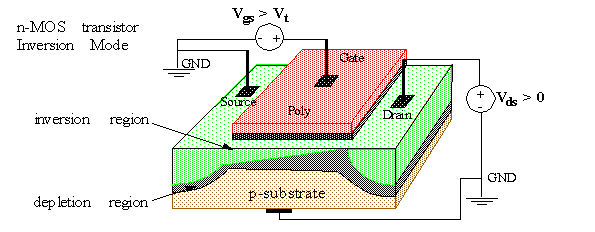
\includegraphics[width=\textwidth]{mos_transistor.png}
		\caption[Corte de transistor MOSFET]{Corte de transistor MOSFET\protect\footnotemark}
		\label{fig:mos_transistor.png}
	\end{figure}

	\footnotetext{Fuente: \url{http://ece-research.unm.edu/jimp/vlsi/slides/chap2_1.html} }
	
	Un transistor MOSFET es un tipo de transistor que se usa para amplificar y conmutar señales eléctricas dentro de un circuito. Se compone de cuatro entradas: fuente, puerta, drenador, y sustrato, que normalmente está conectado a la fuente para evitar la modulación de la tensión de corte. Cuando se aplica un voltaje entre la puerta y la fuente, se crea un canal en el medio semiconductor que permite el paso de corriente entre la fuente y el drenador. Podemos distinguir dos tipos de transistores MOS: los canal-n y los canal-p, dependiendo del dopaje del silicio usado en su fabricación. Los canal-n tienen un dopaje negativo en el silicio de la fuente y el drenador, que se consigue añadiendo impurezas de un elemento como fósforo, dejando electrones libres que actúan como portadores de carga. En el caso de los canal-p, se dopan con elementos como boro, que dejan huecos (ausencia de electrones en capas de valencia), y estos actúan como portadores de carga.
	
	Estos son los símbolos más usados para representar transistores MOS:
	
	\begin{figure}[H]
		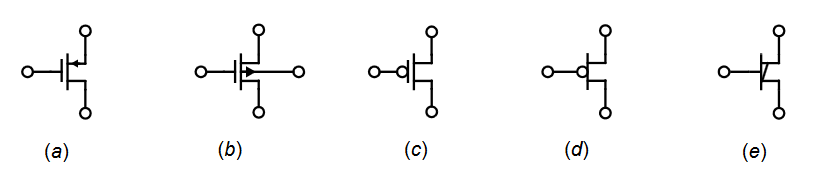
\includegraphics[width=0.8\textwidth]{p-mos-symbol.png}
		\caption[Transistor MOS, canal-p]{Transistor MOS, canal-p\protect\footnotemark}
		\label{fig:p-mos-symbol.png}
	\end{figure}

	\footnotetext{Fuente: \cite{aicd}}
	
	\begin{figure}[H]
		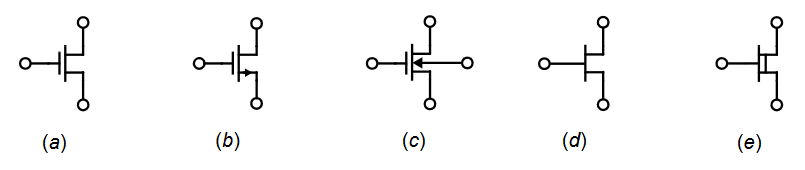
\includegraphics[width=0.8\textwidth]{n-mos-symbol.png}
		\caption[Transistor MOS, canal-n]{Transistor MOS, canal-n\protect\footnotemark}
		\label{fig:n-mos-symbol.png}
	\end{figure}

	\footnotetext{Fuente: \cite{aicd}}

	El comportamiento general de este tipo de transistores se modela a través de regiones de funcionamiento, que dependen del voltaje $V_{GS}$, o voltaje entre puerta y fuente.
	La siguiente tabla describe esta relación para un transistor tipo n. Para un tipo p, las reglas aplican igual, invirtiendo el signo de los voltajes.
	
	\begin{table}[H]
		\begin{tabular}{|c|c|}
			\hline
			$V_{GS}$ & Región \\
			\hline
			$< V_{T}$ & Corte \\
			\hline
			$> V_{DS} + V_{T}$ & Lineal u óhmica \\
			\hline
			$< V_{DS} + V_{T}$ & Saturación o activa \\
			\hline
		\end{tabular}
	\end{table}

	Siendo $V_{T}$ el voltaje límite y $V_{DS}$ el voltaje entre drenador y fuente. El voltaje límite es voltaje mínimo necesario para la aparición de un canal entre la fuente y el drenador. Depende de parámetros de fabricación, como el ancho de la capa de óxido y su material, y de parámetros de funcionamiento, como la temperatura y el voltaje del sustrato (por el llamado \textit{efecto cuerpo}\footnote{El efecto cuerpo relaciona el voltaje de sustrato con el voltaje límite. Un cambio en el voltaje de sustrato conlleva un cambio de similar valor en el voltaje límite.}). %TODO: efecto cuerpo??? comprobar este nombre!
	
	En la región de corte, no existe canal entre fuente y drenador, así que no se permite el paso de corriente entre ambos. En la región lineal u óhmica, el canal aparece, pero ofrece una cierta impedancia al paso de corriente, de tal manera que el transistor se comporta como una resistencia que disminuye según aumenta $V_{GS}$ con respecto a $V_{DS} + V_{T}$. En la región de saturación, o región activa, el canal permite el paso libre de corriente, y deja de ser dependiente de la relación de voltaje entre $V_{GS}$ y $V_{DS} + V_{T}$.
	
	\section{Tecnología CMOS}
	
	La tecnología de fabricación CMOS\footnote{Complementary MOS} utiliza una combinación de transistores MOS de canal n y canal p para implementar las operaciones lógicas. Fue desarrollada en la década de 1960 por empleados de la compañía Fairchild Semiconductor\cite{cmos-fairchild}.
	
	Por ejemplo, un inversor (puerta lógica NOT) se consigue con la siguiente disposición:
	
	\begin{figure}[H]
		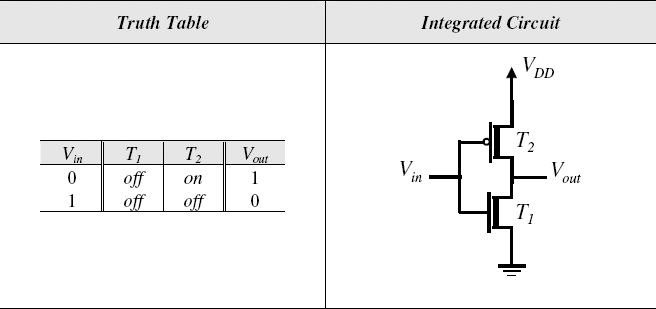
\includegraphics[width=0.75\textwidth]{inverter_mos.jpg}
		\caption[Inversor CMOS]{Inversor CMOS\protect\footnotemark}
		\label{fig:inverter_mos.jpg}
	\end{figure}
	\footnotetext{Fuente: \url{https://www.oreilly.com/library/view/introduction-to-digital/9780470900550/chap5-sec008.html} }
	
	
	Los circuitos CMOS tienen un bajo consumo estático, ya que una vez formado el canal en región activa, la alta impedancia de entrada provoca un paso de corriente casi nulo, únicamente provocado por corrientes parásitas. También tienen una buena tolerancia al ruido por su propiedad regenerativa de la señal: si entra una señal degradada (alejada de su valor nominal) a una puerta CMOS, esta volverá al valor lógico que corresponda, dentro de las tolerancias que permita el circuito. Por estas propiedades es por las que la tecnología CMOS se ha convertido en dominante en el diseño de microcircuitos en la actualidad.
	
	\section{Conversión analógico-digital}
	
	La tarea de un convertidor analógico-digital, o ADC, es tomar una señal eléctrica analógica y transformarla en una digital. Una señal analógica es aquella producida por un fenómeno electromanético y representable por una función continua que define su periodo y amplitud. Una señal digital es una sucesión de diferentes valores discretos con un espaciado temporal uniforme.
	
	\begin{figure}[H]
		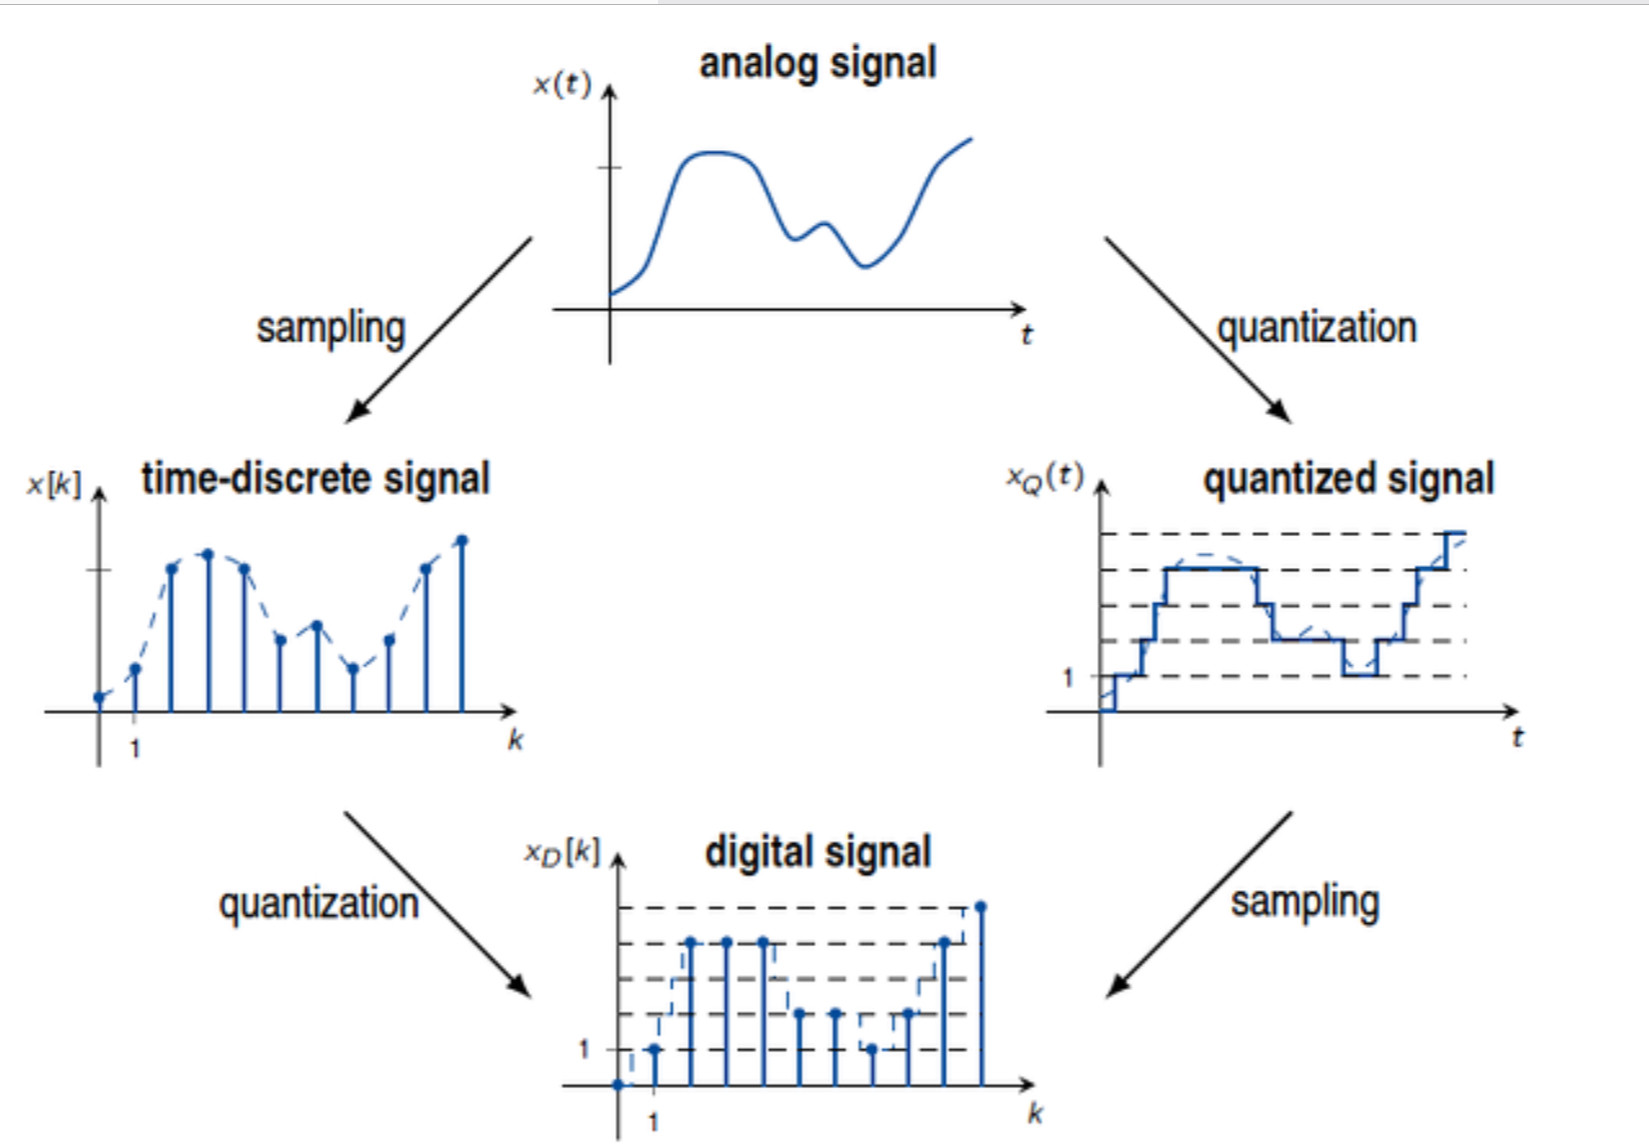
\includegraphics[width=0.75\textwidth]{analog-vs-digital-signal.jpg}
		\caption[Señal analógica a digital]{Señal analógica a digital\protect\footnotemark}
		\label{fig:analog-vs-digital-signal.jpg}
	\end{figure}
	\footnotetext{Fuente: \url{https://electronics.stackexchange.com/questions/352784/in-digital-systems-do-we-discretize-both-time-and-magnitude-or-only-time} }
	
	En un ADC, la señal analógica original sufre dos transformaciones: un muestreo y una cuantificación. El muestro toma valores de la señal a una frecuencia concreta, descartando los intermedios. La cuantificación transforma el espectro continuo de la señal en un conjunto de valores finito. Esto es suficiente para lograr un conjunto de palabras (conjunto de bits de longitud definida) a una frecuencia de trabajo, para ser almacenadas o procesadas por un microcontrolador.
	
	Estos son algunos de los parámetros básicos que describen el comportamiento y prestaciones de un ADC:
	
	\begin{description}[font=\bfseries, style=multiline, align=left, before={\renewcommand\makelabel[1]{\bfseries ##1:}}]
		\item[Frecuencia de muestreo] Frecuencia a la cual se toman medidas de la señal original. Determinado por el ancho de banda de la aplicación.
		\item[Ancho de banda] Rango de frecuencias de la señal original que puede ser correctamente muestreada, cuantizada, y posteriormente recreada. 
		\item[Resolución] Número de pasos máximo entre rango de valores de la señal analógica. Determina el error de cuantificación y el SNR máximo.
		\item[SNR] La Signal-to-Noise Ratio, o Relación Señal-Ruido, es la relación entre la potencia de la señal transmitida y la potencia del ruido presente en dicha señal. Normalmente se representa en dB. 
			\begin{figure}[H]
				\begin{equation}
					\label{snr}
					SNR = \frac{P_{signal}}{P_{noise}}
				\end{equation}
			\end{figure}
			\begin{figure}[H]
				\begin{equation}
					\label{snr-db}
					SNR_{dB} = 10 log_{10} (\frac{P_{signal}}{P_{noise}})
				\end{equation}
			\end{figure}
					
	\end{description}

	En cuanto a errores en la conversión, estas son las principales fuentes:
	
	\begin{description}[font=\bfseries, style=multiline, align=left, before={\renewcommand\makelabel[1]{\bfseries ##1:}}]
		\item[Cuantificación] Para una muestra dada en un momento determinado, es la diferencia entre el valor de la señal original y valor de la señal cuantificada.
		\item[Linealidad] Falta de correlación lineal entre entrada y salida del ADC. Necesita ser corregida para evitar divergencias entre entrada y salida que distorsionan la lectura.
	\end{description}

	Es importante diferenciar dos tipos de ADC según su frecuencia de muestreo:
	\begin{description}[font=\bfseries, style=multiline, align=left, before={\renewcommand\makelabel[1]{\bfseries ##1:}}]
		\item[A frecuencia de Nyquist] La frecuencia de muestreo es igual a dos veces la frecuencia máxima de la señal a capturar\cite{nyquist}\cite{shannon-nyquist}. El teorema de Nyquist habla de esta frecuencia como la mínima a la que es matemáticamente posible recrear una señal perfectamente a partir de las muestras tomadas.
		\item[Sobremuestreados] La frecuencia de muestreo es superior a la frecuencia de Nyquist; habitualmente unas diez veces mayor.
	\end{description}
	
	\section{Arquitecturas de ADC actuales}
	
	Existen multitud de arquitecturas ADC, entre ellas: flash, aproximaciones sucesivas, de integración, de rampa, de seguimiento, tensión-frecuencia. Algunos ejemplos:
	
	\begin{figure}[H]
		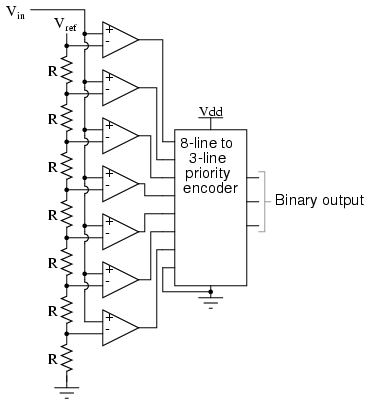
\includegraphics[width=0.5\textwidth]{flash-adc.png}
		\caption[ADC de conversión directa tipo flash]{ADC de conversión directa tipo flash\protect\footnotemark}
		\label{fig:flash-adc.png}
	\end{figure}
	\footnotetext{Fuente: \url{https://www.allaboutcircuits.com/textbook/digital/chpt-13/flash-adc/} }
	\begin{figure}[H]
		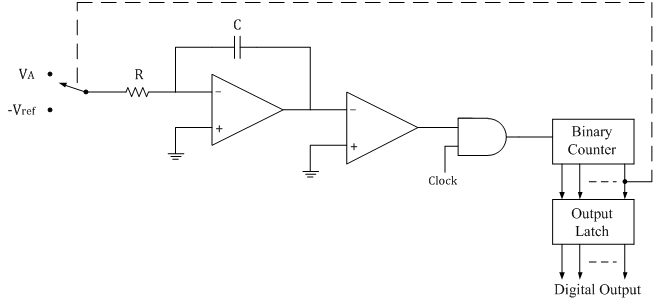
\includegraphics[width=0.6\textwidth]{integrator-adc-double-ramp.png}
		\caption[ADC integrador de doble rampa]{ADC integrador de doble rampa\protect\footnotemark}
		\label{fig:integrator-adc-double-ramp.png}
	\end{figure}
	\footnotetext{Fuente: \url{http://www.electronics-tutorial.net/analog-integrated-circuits/data-converters/dual-slope-type-adc/} }
	
	Los más cercanos a la materia de este estudio son los de integración, en concreto los que utilizan la modulación sigma-delta.
	
	\section{Modulación sigma-delta en ADCs}
	
	Un ADC que utiliza el principio de modulación sigma-delta, también llamado \textit{modulador sigma-delta}, o \textit{modulador \sigmadelta}, tiene como bloques principales un negador, un integrador, y un cuantificador, además de un bucle de realimentación. Este es el esquema de bloques básico de un modulador \sigmadelta:
	
	\begin{figure}[H]
		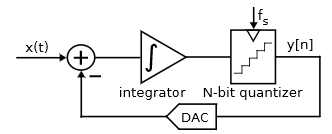
\includegraphics[width=0.6\textwidth]{sigma-delta-blocks.png}
		\caption[Bloques de un modulador \sigmadelta]{Bloques de un modulador \sigmadelta\protect\footnotemark}
		\label{fig:sigma-delta-blocks.png}
	\end{figure}
	\footnotetext{Fuente: Oversampled Analog-To-Digital Converter Architectures Based On Pulse Frequency Modulation\cite{eric-thesis} }
	
	El funcionamiento de este tipo de ADC sigue los pasos siguientes. La señal original $( x(t) )$ es sumada a la salida del cuantificador $( y(t) )$ en magnitud negativa. La salida $( y(t) )$ es un flujo de un bit de profundidad, por lo que debe ser transformada a magnitud real a través de un DAC. El integrador forma un filtro de paso bajo sobre la diferencia entre señal original y cuantificada de tal manera que se consigue una realimentación de baja frecuencia, consiguiendo una reducción del ruido de cuantificación en la banda de respuesta.
	
	Este es un ejemplo gráfico del resultado de la modulación \sigmadelta:
	
	\begin{figure}[H]
		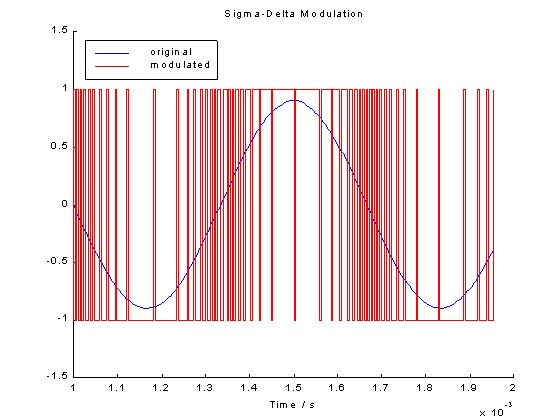
\includegraphics[width=\textwidth]{sd-modulation-example.jpg}
		\caption[Modulación \sigmadelta de una señal de 1.5kHz]{Modulación \sigmadelta de una señal de 1.5kHz\protect\footnotemark}
		\label{fig:sd-modulation-example.jpg}
	\end{figure}

	\footnotetext{Fuente: \url{http://www.cs.tut.fi/sgn/arg/rosti/1-bit/} }
	
	Se puede observar que el promedio de la señal modulada de 1 bit es proporcional a la señal original.
	
	Con respecto a un ADC de aproximaciones sucesivas o de seguimiento, la modulación \sigmadelta una gran linealidad en la curva de respuesta y una disminución del ruido de fondo, ya que el bucle tenderá a hacer que la salida $y(t)$ sea cero. El cuantificador suele ser un comparador implementado con un amplificador operacional de alta ganancia, con una referencia ajustada a la aplicación. Además suele existir un circuito sample-and-hold con una frecuencia de reloj que se ajusta a la entrada al circuito que recibirá la señal ya convertida a digital.
	
	En cuanto al integrador, las implementaciones más comunes son con un amplificador operacional o por transconductancia.
	
	\begin{figure}[H]
		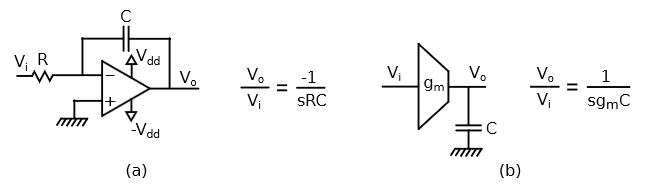
\includegraphics[width=\textwidth]{integrator-opamp-trans.png}
		\caption[Integradores por opamp (a) y por transconductancia (b)]{Integradores por opamp (a) y por transconductancia (b)\protect\footnotemark}
		\label{fig:integrator-opamp-trans.png}
	\end{figure}
	
	\footnotetext{Fuente: \cite{eric-thesis} }
	
	Como se puede observar, ambas opciones trabajan en ámbito analógico.
	
	Las principales desventajas de la conversión por modulador \sigmadelta son la necesidad de una frecuencia de muestreo muy alta respecto a la original, lo cual es un problema a la hora de convertir señales de muy alta frecuencia, y que gran parte del circuito funciona con señales analógicas, lo que complica la implementación en arquitecturas de muy bajo tamaño
	
	\section{VCO en anillo}
	
	Un VCO, siglas de \textit{Voltage Controlled Oscillator} es un componente electrónico que emite un tren de pulsos cuya frecuencia es proporcional a un voltaje de entrada.
	
	Un VCO en anillo es un tipo de oscilador controlado por voltaje. En su forma más básica, consiste en un número impar de puertas inversoras colocadas en un bucle cerrado. En las entradas de alimentación de las puertas se conecta la señal a modular. Este señal de entrada puede ser en voltaje o, a través de un transconductor, en corriente. La señal ya modulada aparece entre la salida y la entrada de cualquier par de puertas.
	
	Esta es la representación simbólica de una puerta inversora, con sus conexiones nombradas:
	\begin{figure}[H]
		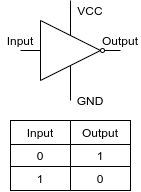
\includegraphics[width=0.3\textwidth]{inverter-symbol.png}
		\caption[Símbolo y tabla de verdad de una puerta inversora]{Símbolo y tabla de verdad de una puerta inversora}
		\label{fig:inverter-symbol.png}
	\end{figure}
	
	Así se consigue un inversor en tecnología CMOS. El transistor superior es de canal-p, y el inferior es de canal-n.
	\begin{figure}[H]
		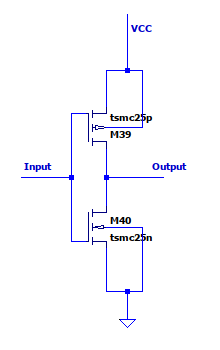
\includegraphics[width=0.4\textwidth]{inverter-sch.png}
		\caption[Esquemático de una puerta inversora con transistores MOS]{Esquemático de una puerta inversora con transistores MOS}
		\label{fig:inverter-sch.png}
	\end{figure}
	
	La siguiente tabla expone el régimen de funcionamiento de ambos transistores, atendiendo a la señal entrada:
	
	\begin{table}[H]
		\begin{tabular}{|c|c|c|c|}
			\hline
			input & Canal-n & Canal-p & output\\
			\hline
			0 & Corte & Activo & $V_{cc}$ \\
			\hline
			$V_{i}$ & Activo & Corte & 0 \\
			\hline
		\end{tabular}
	\end{table}
	
	Donde $V_i$ es un valor que cumple $V_{GS} < V_{DS} + V_{T}$ para ambos transistores, normalmente algo cercano a $V_{cc}$.
	
	Esta es la configuración de puertas para lograr un VCO:
	
	\begin{figure}[H]
		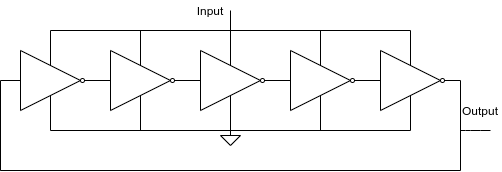
\includegraphics[width=\textwidth]{vco-symbol.png}
		\caption[VCO compuesto por 5 puertas inversoras]{VCO compuesto por 5 puertas inversoras}
		\label{fig:vco-symbol.png}
	\end{figure}
	
	\begin{figure}[H]
		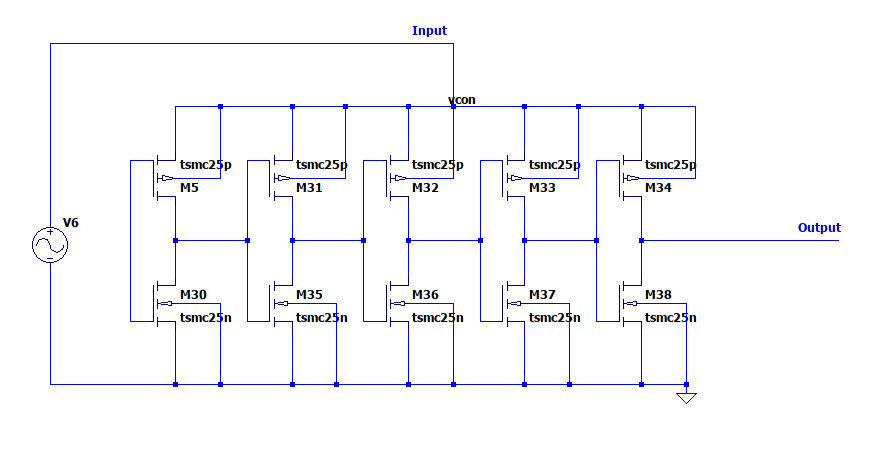
\includegraphics[width=\textwidth]{vco-sch.png}
		\caption[Esquemático de un VCO]{Esquemático de un VCO}
		\label{fig:vco-sch.png}
	\end{figure}
	
	El número impar de puertas inversoras provoca un estado de inestabilidad en el oscilador. Hay una pequeña demora en la activación de las puertas por efecto de las corrientes parásitas, que retrasan el cambio de voltaje, y por tanto el cambio de región de operación del transistor. La realimentación positiva en el anillo hace que se creen señales alternativas entre un 1 lógico y un 0 lógico entre la entrada y la salida de cada puerta. La frecuencia a la que estas señales cambian es proporcional al voltaje aplicado en la alimentación de las puertas (VCC en la figuras \ref{fig:inverter-symbol.png} y \ref{fig:inverter-sch.png}). La frecuencia de oscilación sigue la siguiente fórmula:
	
	\begin{figure}[H]
		\begin{equation}
			\label{vco-freq-sw-t}
			f = \frac{1}{2 n \tau}
		\end{equation}
		\footnotemark
	\end{figure}
	\footnotetext{Fuente: \cite{eric-thesis}}
	
	Donde $n$ es el número de puertas en el anillo y $\tau$ es el retraso de activación de la puerta, que es inversamente proporcional a la señal de entrada. Por ello, $f$ depende la señal de entrada.
	
	Asumiendo un comportamiento ideal del VCO, podemos expresar la relación entre entrada y salida como:
	\begin{figure}[H]
		\begin{equation}
			\label{vco-freq-ideal}
			f_{VCO}= f_{0} + K_{VCO} * V_{i}
		\end{equation}
		\footnotemark
	\end{figure}
	\footnotetext{Fuente: \cite{eric-thesis}}
	
	Donde $f_{VCO}$ es la frecuencia del oscilador, $f_{0}$ es la frecuencia en reposo (con una señal de entrada equivalente a 0), $K_{VCO}$ es la ganancia intrínseca en $Hz/V$, y $V_{i}$ es el valor de voltaje de entrada.
	
	Viendo el oscilador como un integrador, y tomando la fase de la señal como salida, en vez de la frecuencia, hacemos el siguiente análisis:
	
	\begin{figure}[H]
		\begin{equation}
			\label{vco-phase}
			\theta(t) = 2\pi\int_{0}^{t}f_{VCO}(\tau)d\tau = 2\pi f_{0}t + 2\pi K_{VCO}\int_{0}^{t}x(\tau)d\tau
		\end{equation}
		\footnotemark
	\end{figure}
	\footnotetext{Fuente: \cite{eric-thesis}}
	
	Haciendo un análisis en frecuencia, la transformada de laplace del oscilador resulta así:
	
	\begin{figure}[H]
		\begin{equation}
			\label{vco-laplace}
			\frac{2 \pi K_{VCO}}{s}
		\end{equation}
		\footnotemark
	\end{figure}
	\footnotetext{Fuente: \cite{eric-thesis}}
	
	
	Como se puede observar, la señal que entra al oscilador es analógica, mientras que la que sale ya es digital, aunque debe ser demodulada más tarde. Con pocos componentes, se consigue un integrador y cuantificador que funciona principalmente en el ámbito digital, evitando las restricciones que supone el procesado de una señal analógica, como se comentó en la introducción. De aquí surge el interés de los osciladores en anillo en su uso en ADCs.
	
	\section{Osciladores en anillo en ADCs}
	
	\subsection{Como parte de arquitecturas ya existentes}
	Ya que estos osciladores actúan como un integrador, pueden usarse en arquitecturas de ADC ya establecidas, como los \sigmadelta.
	
	Este es un ejemplo de un modulador \sigmadelta de segundo orden con un VCO en anillo sustituyendo el segundo integrador y el cuantificador.
	\begin{figure}[H]
		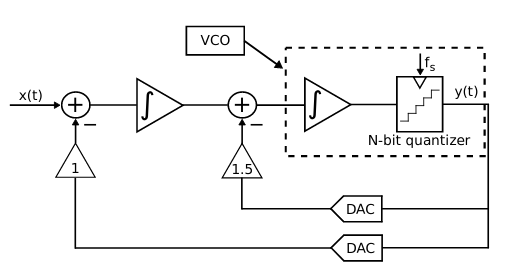
\includegraphics[width=0.7\textwidth]{sd-with-vco.png}
		\caption[Modulador \sigmadelta con un VCO]{Modulador \sigmadelta con un VCO\protect\footnotemark}
		\label{fig:sd-with-vco.png}
	\end{figure}
	\footnotetext{Fuente: \cite{eric-thesis}}
	
	En rendimiento es equivalente a una implementación habitual con opamps, pero con menor consumo y número de componentes. %TODO: corroborar con eric
	
	\subsection{Arquitecturas con solo oscilador en anillo}
	
	Además de la integración, un VCO en anillo también se encarga de la cuantificación. Así, se puede obtener un ADC con solo este componente.
	
	La forma más básica consiste en solo un VCO con un circuito sample-and-hold y un circuito para sacar la primera diferencia.
	\begin{figure}[H]
		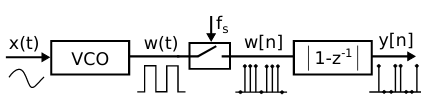
\includegraphics[width=0.6\textwidth]{vco-adc-open-loop.png}
		\caption[ADC con VCO en bucle abierto]{ADC con VCO en bucle abierto\protect\footnotemark}
		\label{fig:vco-adc-open-loop.png}
	\end{figure}
	\footnotetext{Fuente: \cite{eric-thesis}}
	
	Haciendo un análisis en frecuencia de este sistema, tenemos:
	\begin{figure}[H]
		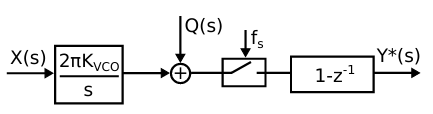
\includegraphics[width=0.6\textwidth]{vco-adc-open-loop-lp.png}
		\caption[Sistema con bucle abierto]{Sistema con bucle abierto\protect\footnotemark} %TODO: mejor nombre para esto
		\label{fig:vco-adc-open-loop-lp.png}
	\end{figure}
	\footnotetext{Fuente: \cite{eric-thesis}}
	
	\begin{figure}[h]
		\begin{equation}
			\label{vco-open-loop-laplace}
			Y(s)=2\pi K_{VCO}X(s) + (1 - z^{-1})Q(s)
		\end{equation}
	\end{figure}
	
	Donde $Q$ es el ruido de cuantificación del VCO, que se modela como una señal aleatoria aditiva a la salida del VCO.
	
	Aunque el rendimiento de esta configuración es similar a los \sigmadelta convencionales, el VCO aporta un gran problema: la curva de respuesta voltaje-frecuencia no es lineal, porque el tiempo de activación de las puertas (ecuación \ref{vco-freq-sw-t}) varía en función de la alimentación de las puertas; en el caso de un oscilador en anillo, esta alimentación es la señal a modular. Esto provoca distorsión en la cuantificación, con lo que se pierde en resolución en el muestreo.
	
	Las soluciones más comunes a este problema son:
	
	\begin{itemize}
		\item Calibración Digital: Se hace un análisis de la curva de respuesta, se crea una tabla de mapeo entrada-salida, y por se hace la corrección por interpolación en un circuito digital. Aumenta mucho el área ocupada y el consumo.
		
		\item Modulación previa al VCO: Se coloca un modulador, habitualmente de tipo PWM, para limitar la frecuencia de oscilación de la señal que entra en el VCO. Es una solución más sencilla, pero el modulador PWM consume mucho y puede presentar no linealidad, así que el problema se mueve de componente, pero no se elimina de todo el sistema.
		
		\item Reducción de la señal de entrada: Si se consigue lo suficiente, se reduce el impacto de la amplitud de la señal en la linealidad del sistema. Algunas maneras usadas para esto son la inclusión de un ADC más básico antes del VCO, cuya señal se resta a la entrada. Así se consigue disminuir la amplitud de la señal que entra al VCO. Este método necesita de un ADC extra, con el consecuente aumento en consumo y espacio ocupado.
		
		\item Ajuste por circuito: Ajustando individualmente la alimentación de las puertas con componentes pasivos se puede paliar la no linealidad, pero esta técnica pierde fiabilidad una vez se toman en cuenta los errores de fabricación, la temperatura, y pequeñas variaciones en voltaje de alimentación.
	\end{itemize}
	
	Ninguna de las soluciones anteriores es perfecta. %TODO: terminar esto
	
\chapter{Propuesta realizada}
	
	En este capítulo se expone el análisis de una nueva arquitectura de ADC que emplea un VCO como cuantificador e integrador, usando un lazo de realimentación negativo para linealizar la respuesta del VCO.
	
	\section{Idea inicial}\label{sc:initial-idea}
	
	La idea fundamental de esta nueva arquitectura es, partiendo de un sistema de ADC por VCO en bucle abierto, estudiar la viabilidad de linealizar la respuesta mediante un bucle de realimentación, haciendo uso de la ganancia intrínseca de la dispone el propio oscilador. Esto eliminaría la necesidad de un amplificador operacional presente en las arquitecturas de VCO con realimentación existentes hoy en día, rebajando por tanto el número de componentes necesarios y el consumo total del sistema.
	
	La idea principal de esta arquitectura viene de publicaciones que ya hacen uso de un bucle de realimentación con DAC de 1 bit controlado por frecuencia. En esta publicación: \textit{VCO-ADC linearization by switched capacitorfrequency-to-current conversion}\cite{vco-adc-ruben-eric} ya se destacan los beneficios de un ADC por VCO con realimentación, como son una mayor resistencia al ruido por jitter del reloj, mayor resistencia al ruido térmico de los componentes pasivos, y una mejora importante de la relación señal-ruido con respecto a un ADC VCO en bucle abierto. El problema de la arquitectura propuesta en la publicación es que no consigue prescindir de un amplificador operacional, que sigue siendo el componente más complejo, costoso, y con gran consumo.
	
	En este estudio, exploraremos la posibilidad de usar la ganancia intrínseca del VCO para poder eliminar el amplificador operacional, para reducir el consumo y el tamaño del ADC, y abrir su uso a nuevas aplicaciones que requieren de una gran miniaturización y eficiencia.
	
	
	\section{Análisis matemático del VCO con realimentación negativa}
	
	Una manera común de linealizar un sistema es con un bucle de realimentación negativa. Partiendo de un ADC con VCO en bucle abierto, la manera más sencilla de incluir realimentación es unir la salida con la entrada a través de un sumador. En el bucle debe existir una conversión de la salida digital del VCO a la entrada analógica del sistema.

	\begin{figure}[H]
		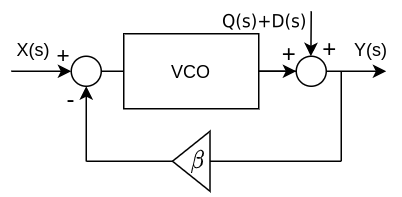
\includegraphics[width=0.5\textwidth]{vco-diagram-closed-loop-with-D.png}
		\caption[ADC con VCO en bucle abierto, diagrama de bloques]{ADC con VCO en bucle cerrado, diagrama de bloques}
		\label{fig:vco-diagram-closed-loop-with-D.png}
	\end{figure}
	
	Haciendo un análisis del sistema, podemos despejar la función de transferencia del sistema:
	
	\begin{figure}[H]
		\caption{Desarrollo de la función de transferencia del VCO con lazo cerrado}
		\label{vco-closed-loop-s}
		\begin{equation}
		\begin{array}{lcl}
		VCO & : & \frac{K_{VCO}}{s} \\
		Y(s) &=& ( Q(s) + D(s) ) + \frac{K_{VCO}}{s}(X(s) - \beta Y(s) ) \\
		Y(s) &=& ( Q(s) + D(s) ) + \frac{K_{VCO}}{s}X(s) - \frac{K_{VCO} \beta}{s}Y(s) \\
		Y(s) (1 + \frac{K_{VCO}\beta}{s}) &=& ( Q(s) + D(s) ) + \frac{K_{VCO}}{s}X(s) \\
		Y(s) (\frac{s + K_{VCO}\beta}{s}) &=& ( Q(s) + D(s) ) + \frac{K_{VCO}}{s}X(s) \\
		Y(s) &=& \frac{s}{s + K_{VCO}\beta}( Q(s) + D(s) ) + \frac{K_{VCO}}{s + K_{VCO}\beta}X(s) \\
		\end{array}
		\end{equation}
	\end{figure}
	
	Donde $Y(s)$ es la señal de salida, $X(s)$ es la señal de entrada, $K_{VCO}$ es la ganancia del VCO, $\beta$ es la ganancia del lazo de realimentación, y $( Q(s) + D(s) )$ es el ruido de cuantificación y el ruido de no linealidad, respectivamente, modelados como señales que se suman a la salida del VCO.
	
	Respecto a los términos a la derecha de la ecuación superior, podemos deducir el siguiente comportamiento del sistema en función de la frecuencia:
	
	\begin{figure}[H]
		\label{vco-closed-loop-terms-x}
		\begin{equation}
		\begin{array}{lcl}
		\frac{K_{VCO}}{s + K_{VCO}\beta}X(s) & \\
		\frac{K_{VCO}}{s + K_{VCO}\beta}, s \to \infty: & = 0 \\
		\frac{K_{VCO}}{s + K_{VCO}\beta}, s \to 0: & = \frac{1}{\beta} \\
		\end{array}
		\end{equation}
	\end{figure}

	\begin{figure}[H]
		\label{vco-closed-loop-terms-q}
		\begin{equation}
		\begin{array}{lcl}
		\frac{s}{s + K_{VCO}\beta}Q(s) & \\
		\frac{s}{s + K_{VCO}\beta}, s \to 0: & = \frac{1}{\beta} \\
		\frac{s}{s + K_{VCO}\beta}, s \to \infty: & = 0 \\
		\end{array}
		\end{equation}
	\end{figure}

	Así, tenemos que a altas frecuencias, el coeficiente de $Q(s)$ aumenta y el de $X(s)$ disminuye. A bajas frecuencias, ocurre lo contrario. Por lo tanto, este sistema aplica un filtro paso alto a $Q(s)$ y un filtro paso bajo a $X(s)$. Esto discrimina el ruido de cuantificación y el de linealidad en la banda de frecuencias de la señal de entrada. Para aumentar la SNR\footnote{Signal to Noise Ratio: ratio entre la señal y el ruido} necesitamos pues un valor alto de ganancia $\beta$ en la realimentación, para que este filtro paso bajo tenga mayor magnitud y mayor potencia.
	
	En cuanto a la linealidad del sistema: partimos de un DAC que recoge la frecuencia de salida del VCO y la convierte en corriente. Asumimos que esta conversión es lineal. Esta corriente se resta a la entrada. Integrando esta diferencia (a través del VCO), tiende a cero. Cuando la resta es cero, las señales de entrada y del bucle son iguales, y si la corriente que sale del DAC es lineal con respecto a la frecuencia es lineal, con lo que la corriente de entrada del sistema también es lineal.  Así que consiguiendo un DAC que realice la conversión con un buen nivel de linealidad dentro del ancho de banda de interés, resolvemos el problema de la linealidad en el VCO.
	
	\subsection{Lazo de realimentación por capacidades conmutadas}
	
	Dado que la ganancia del VCO es relativamente estable y más compleja de manipular, en este estudio nos centramos en la ganancia en el lazo de realimentación. En el lazo es necesario hacer una conversión de la señal modulada digital, a la señal de entrada analógica. Para esto es necesario buscar un DAC relativamente sencillo para no volver a encontrarnos el problema que intentamos evitar: número de componentes y consumo. Además, los requisitos para el DAC no son especialmente restrictivos, salvo que la transformación sea lineal.
	
	
	La solución escogida es el uso de un sistema de capacidades conmutadas. En nuestra implementación, este se compone de dos transistores pareados CMOS, en una distribución casi idéntica a las puertas lógicas inversoras.
	
	\begin{figure}[H]
		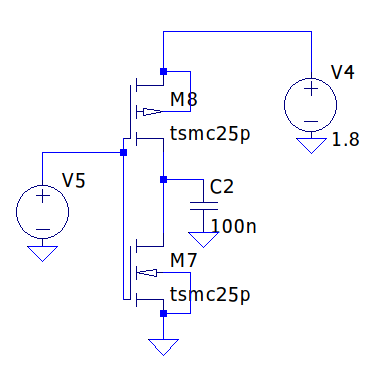
\includegraphics[width=0.6\textwidth]{sw-capacities-sch.png}
		\caption[Esquemático de circuito de capacidades conmutadas]{Esquemático de circuito de capacidades conmutadas}
		\label{fig:sw-capacities-sch.png}
	\end{figure}
	
	El circuito consta de dos transistores CMOS, canal-n y canal-p, y un condensador conectado entre fuente y drenador de los transistores. La fuente de alimentación $V4$ se conecta a la fuente del transistor canal-p, y la señal modulada en FM\footnote{Frequency Modulation, modulación en frecuencia.} se conecta a las puertas de ambos transistores. La señal PFM actúa a modo de reloj para controlar la activación de los transistores, que actúan a modo de interruptores.
	
	Este es el diagrama simbólico del sistema:
	
	\begin{figure}[H]
		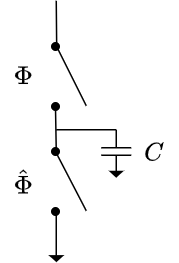
\includegraphics[width=0.3\textwidth]{sw-capacities-symbol-1.png}
		\caption[Diagrama de circuito de capacidades conmutadas]{Diagrama de circuito de capacidades conmutadas}
		\label{fig:sw-capacities-symbol-1.png}
	\end{figure}

	Donde $\Phi$ es una señal de reloj de frecuencia variable y $\hat{\Phi}$ es la inversa del mismo reloj.
	
	A continuación se presenta un análisis del comportamiento en función del valor del reloj:
	
	\begin{figure}[H]
		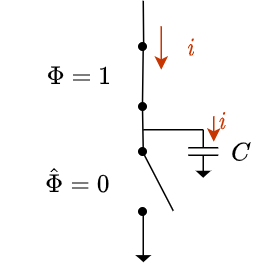
\includegraphics[width=0.4\textwidth]{sw-capacities-symbol-2.png}
		\caption[Diagrama para $\Phi=1$]{Diagrama para $\Phi=1$}
		\label{fig:sw-capacities-symbol-2.png}
	\end{figure}
	Para $\Phi = 1$ y $\hat{\Phi} = 0$, el transistor superior se activa cerrando el circuito, y el inferior se desactiva abriéndolo. Esto permite el paso de corriente momentáneo al condensador $C$, que durante este semiperiodo se carga.
	
	\begin{figure}[H]
		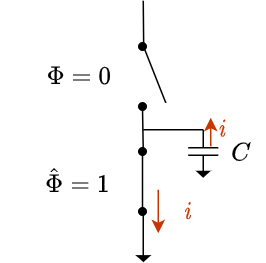
\includegraphics[width=0.4\textwidth]{sw-capacities-symbol-3.png}
		\caption[Diagrama para $\Phi=0$]{Diagrama para $\Phi=0$}
		\label{fig:sw-capacities-symbol-3.png}
	\end{figure}
	Para $\Phi = 0$ y $\hat{\Phi} = 1$, el transistor superior se desactiva abriendo el circuito mientras que el inferior se cierra conectando el condensador con la tierra. Así, se crea un flujo de corriente desde el condensador que lo descarga.
	
	Las siguientes ecuaciones describen la corriente de salida en función de la frecuencia.
	
	\begin{figure}[H]
		\caption{Ecuaciones de corriente de salida en función de la frecuencia para el el DAC por capacidades conmutadas}
		\label{sw-capacities-eqs}
		\begin{equation}
		\begin{array}{c}
		I_C = \frac{\Delta Q}{\Delta t} = \\
		= \frac{C(V_{A}-V_{B})}{T} = Cf(V_{A}-V_{B}) \\
		si\ \ V_{A} = V_{dd}\ \ y\ \ V_{B} = V_{GND} = 0 \implies I_C = Cf(V_{dd})
		\end{array}
		\end{equation}
	\end{figure}
	
	Donde $I_C$ es la corriente media que pasa por el condensador.
	
	Teniendo corriente equivalente y voltaje de referencia, podemos modelar el sistema como una impedancia variable.
	
	\begin{figure}[H]
		\label{sw-capacities-var-res}
		\begin{equation}
		\begin{array}{c}
		Z_{eq} = \frac{V_{dd}}{I_C} = \frac{V_{dd}}{Cf(V_{dd})} = \frac{1}{fC} \\
		\end{array}
		\end{equation}
	\end{figure}
	
	Así obtenemos una resistencia variable proporcional a la frecuencia de entrada, con la que podemos obtener la corriente proporcional a la frecuencia del VCO para nuestro bucle de realimentación.
	
	Debemos tener en cuenta que los transistores tienen unas ciertas corrientes parasíticas fuera de su modelo ideal. Estas corrientes provocan que un transistor abierto tenga una impedancia muy alta, pero no cero, y uno cerrado tenga una impedancia muy baja, pero nunca nula. Relacionando este paso de corriente por los transistores con un voltaje de referencia, podemos modelar los efectos parasíticos como una impedancia intrínseca en los transistores.
	
	Este es el circuito equivalente:
	\begin{figure}[H]
		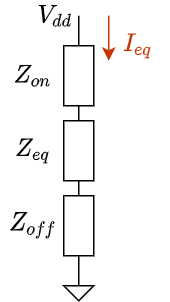
\includegraphics[width=0.2\textwidth]{sw-capacities-var-res-block.png}
		\caption[Diagrama de bloques del sistema de impedancias equivalente]{Diagrama de bloques del sistema de impedancias equivalente}
		\label{fig:sw-capacities-var-res-block.png}
	\end{figure}
	
	Donde $Z_{eq}$ es la impedancia variable equivalente, y $Z_{on}$ y $Z_{off}$ son las impedancias de transistor activado y en corte. Como se abren y cierran de manera alternativa, y asumiendo un comportamiento ideal del sistema (activación/desactivación instantánea, sin solapamiento), el circuito equivalente tendrá una impedancia de cada en serie. Estas impedancias de los transistores dependen de factores como tecnología de fabricación, tamaño, y defectos de fabricación. En cualquier caso, $Z_{on}$ es muy bajo, y $Z_{off}$ es muy alto.
	
	Queda este modelo ideal para el DAC por capacidades conmutadas:
	
	\begin{figure}[H]
		\label{sw-capacities-i_eq}
		\begin{equation}
		\begin{array}{c}
		I_{eq} = \frac{V_{dd}}{\frac{1}{fC} + Z_{on} + Z_{off}} \\
		\end{array}
		\end{equation}
	\end{figure}
	
	Con esto, ya tenemos nuestro DAC que transforma la señal modulada en frecuencia de 1 bit de manera sencilla y con pocos componentes.
	
	\section{Simulaciones del modelo}
	
	Tras el análisis matemático expuesto en las secciones anteriores, procedemos a realizar simulaciones para comprobar la validez de la arquitectura. Usaremos LTSpice para elaborar esquemáticos y lanzar simulaciones, y Matlab/Octave para analizar los resultados.
	
	En estas simulaciones se han usado las librerías de transistores CMOS de la compañía TSMC, cedidas al Departamento de Tecnologías Electrónicas. Estas librerías tienen los parámetros necesarios para poder simular su comportamiento en un programa SPICE.
	
	\subsection{Herramientas de simulación}
	
	\subsubsection{Reloj de frecuencia variable en LTSpice}
	Para conseguir la curva de respuesta un sistema, podemos hacerlo por interpolación, tomando varios resultados discretos para diferentes valores de entrada, en este caso, frecuencia de reloj, o podemos usar una entrada que incremente su valor de forma lineal con el tiempo. Como no existe un componente con este comportamiento en LTSpice, se ha creado uno nuevo:
	
	\begin{figure}[H]
		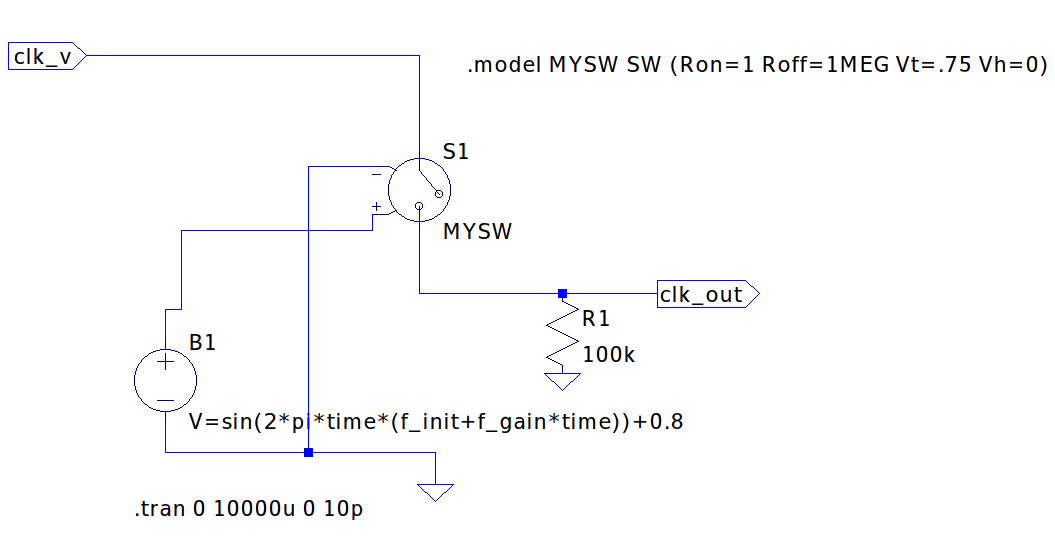
\includegraphics[width=0.8\textwidth]{ltspice-clk-freq.png}
		\caption[Esquemático de reloj con frecuencia incremental]{Esquemático de reloj con frecuencia incremental}
		\label{fig:ltspice-clk-freq.png}
	\end{figure}
	
	Este componente utiliza un interruptor y una fuente de voltaje cuyo valor se calcula con una función sinusoidal en función del tiempo.
	\begin{figure}[H]
		\label{sw-capacities-v_eq}
		\begin{equation}
		\begin{array}{c}
		V=sin(2*\pi*t*(f_{init}+f_{gain}*t))+V_{offset}
		\end{array}
		\end{equation}
	\end{figure}
	
	Donde $t$ es el tiempo en cada paso de la simulación, $f_{init}$ es la frecuencia en $t=0$ del sistema, $f_{gain}$ es un parámetro que dicta el incremento de la frecuencia por unidad de tiempo, y $V_{offset}$ es el voltaje medio de la fuente. Las entrada de este circuito es $f_{gain}$ y el voltaje nominal del reloj $clk\_v$. Además, para que el 0 lógico del reloj tenga un voltaje igual a cero, hay una resistencia \textit{pull-down} justo antes de la salida.
	
	Para comprobar que el componente funciona, a continuación se presenta una simulación rápida. Los valores de las variables para esta simulación son los siguientes:
	\begin{table}[H]
		\label{tab:parameters-clk-freq-sim}
		\caption{Parámetros de simulación del reloj de frecuencia incremental}
		\begin{tabular}{lr}
			clk\_v & 1V \\
			f\_init & 3e3 \\
			f\_gain & 3e7 \\
			Paso de simulación & 1ns \\
			Tiempo de simulación & 10ms
		\end{tabular}
	\end{table}

	Este es el resultado de la simulación:
	
	\begin{figure}[H]
		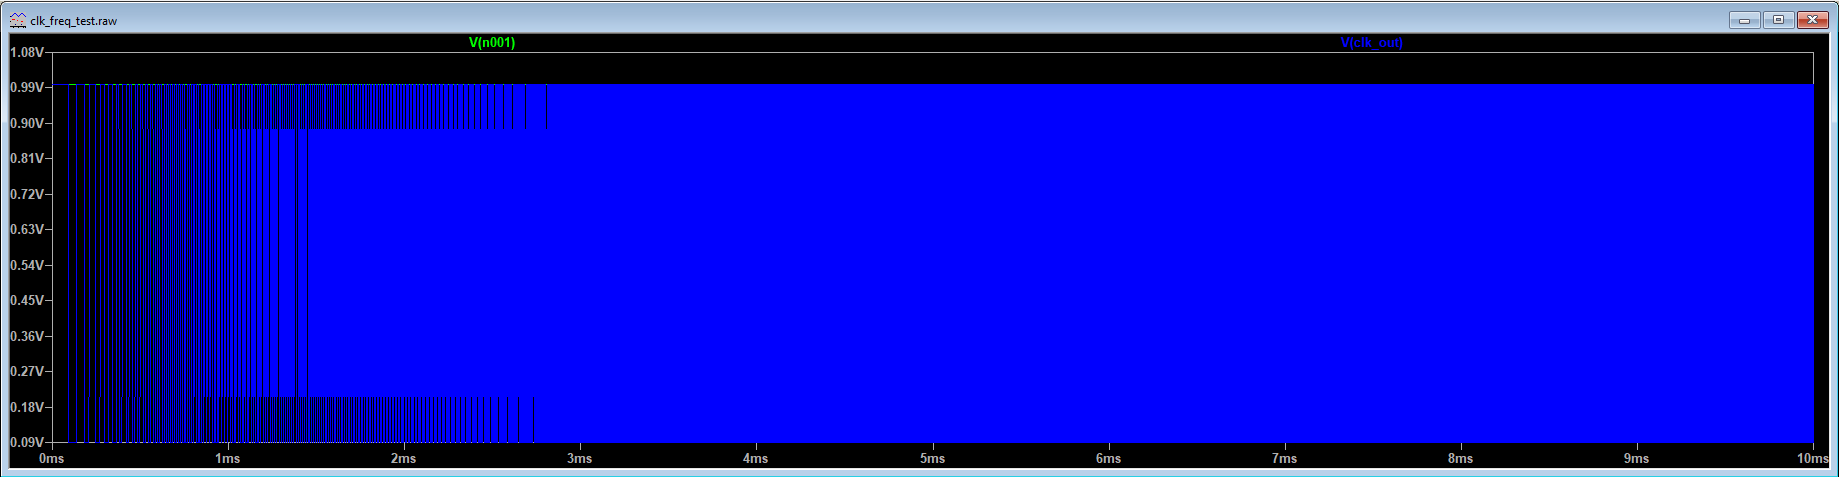
\includegraphics[width=1\textwidth]{clk-freq-sim-waveform.PNG}
		\caption[Simulación: Forma de onda del voltaje en la salida clk\_out]{Simulación: Forma de onda del voltaje en la salida clk\_out}
		\label{fig:clk-freq-sim-waveform.PNG}
	\end{figure}
	
	Se puede observar que la forma de onda del reloj es cuadrada, y va aumentando según pasa el tiempo de simulación. Haciendo zoom en una zona cualquiera, y tomando medidas, podemos calcular la frecuencia de reloj en función de $1/T$:

	\begin{figure}[H]
		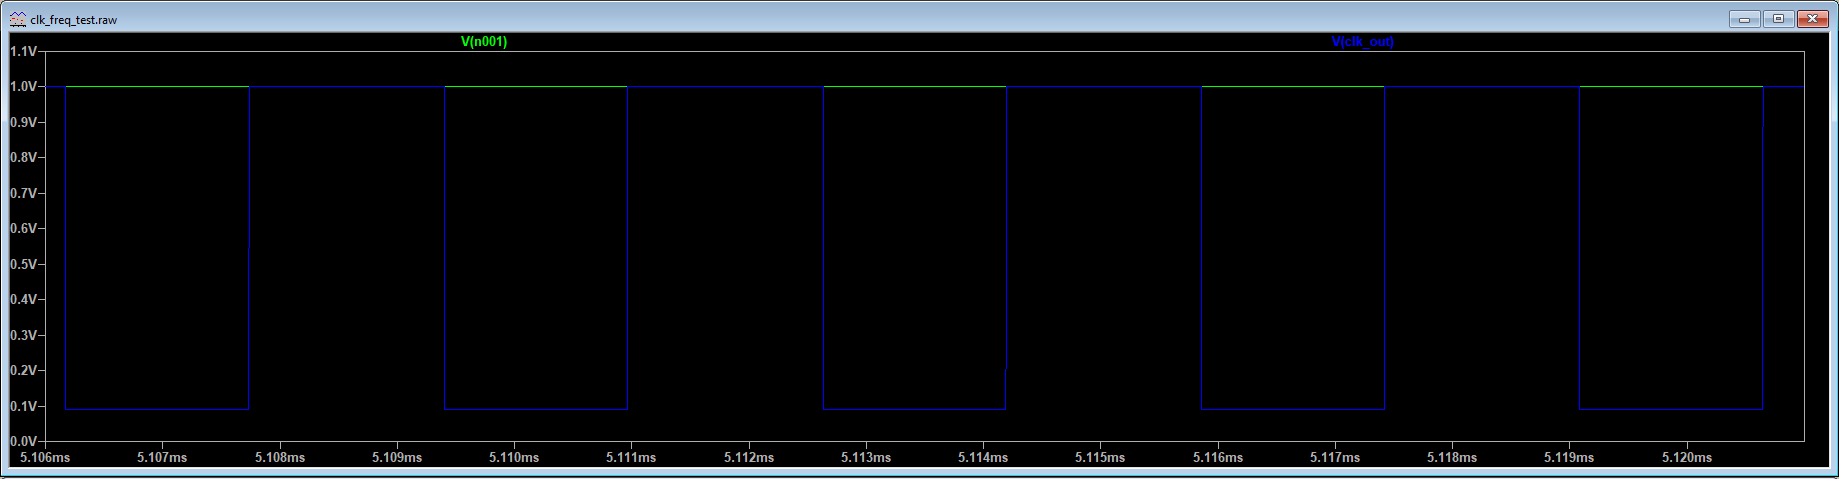
\includegraphics[width=1\textwidth]{clk-freq-sim-waveform-zoom.PNG}
		\caption[Simulación: zoom en sección de la forma de onda]{Simulación: zoom en sección de la forma de onda}
		\label{fig:clk-freq-sim-waveform-zoom.PNG}
	\end{figure}
	
	En esta sección, el periodo es aproximadamente $T=3.2us$. Las ecuaciones que describen la frecuencia real como la teórica son las siguientes:
	
	\begin{figure}[H]
		\begin{equation} \label{eq:clk-freq_eqs_freq}
		\begin{array}{c}
		Real:\; f = \frac{1}{3.2e-6} = 312.5kHz \\
		Te\acute{o}rico:\; time\approx5.111e-3 \implies f = (3e3 + 3e7 * time) = 156.3kHz \\
		\end{array}
		\end{equation}
	\end{figure}

	A la vista queda una cierta discrepancia entre valores. Esto se debe a falta de precisión absoluta en la simulación, y a errores en la toma de medidas de manera visual.
	
	Es necesario un método que permita el análisis de los datos de manera programática, y no manual. Ya que LTSpice permite exportar las formas de onda como matriz de puntos x-y, podemos usar Matlab/Octave para el análisis.
	
	\subsubsection{Procesado de formas de onda en Matlab/Octave}
	
	Partiendo de la matriz de puntos x-y (voltaje-tiempo) de la simulación del apartado anterior, nuestro objetivo es producir una recta frecuencia-tiempo.
	
	Para calcular el periodo en función del tiempo, hacemos una función que guarde el tiempo en que cada periodo comienza, atravesando un threshold, y con el periodo calcularemos su inversa, que es la frecuencia.
	
	Encontramos un problema al analizar el dataset: el paso de simulación es variable, lo que significa que los puntos no están uniformemente espaciados con respecto al tiempo, así que primero debemos limpiar estos datos. Generamos un vector de tiempos con el rango del dataset de simulación, e interpolamos los datos originales para sacar el valor de V que corresponde a cada tiempo. Esto genera un cierto error de resolución %TODO: qué tipo de error es?
	, pero veremos que para nuestro caso es despreciable.
	
	Este es el algoritmo que define el comportamiento del script de procesado:
	
	\begin{lstlisting}[caption={Código en Matlab/Octave para procesar la forma de onda del reloj de frecuencia variable},label={lst:code-clk-var}]
dataset = load(file_name, "-ascii");
length_dataset = length(dataset);
times_eq_spaced = linspace(0, dataset(end,1), length_dataset);
dataset_eq_spaced(:) = interp1(dataset(:,1),dataset(:,2),times_eq_spaced);
timestamp_periods = [];
threshold = 0.8;
for i = 2:length(dataset_eq_spaced)
	if ( dataset_eq_spaced(i) > threshold ) && ( dataset_eq_spaced(i-1) < threshold )
		timestamp_periods = [ timestamp_periods; i t(i) dataset_eq_spaced(i) ];
	end
end
freqs = [];
for i = 1:length(timestamp_periods)
	if i == 1
		freqs(i) = ( 1/( timestamp_periods(i,2) - 0 ) );
	else
		freqs(i) = ( 1/( timestamp_periods(i,2) - timestamp_periods(i-1,2) ) );
	end
end
freqs_ordered = sort(freqs);
plot(Tperiods(:,2), freqs_ordered)
	\end{lstlisting} 
	%TODO: aquí hay trampilla: por algún motivo la frecuencia sale el doble de lo teórico, así que donde pone 1/T, en el script puse 0.5/T

	Este es el resultado del análisis con el dataset de la simulación \ref{fig:clk-freq-sim-waveform.PNG}:
	
	\begin{figure}[H]
		\centerline{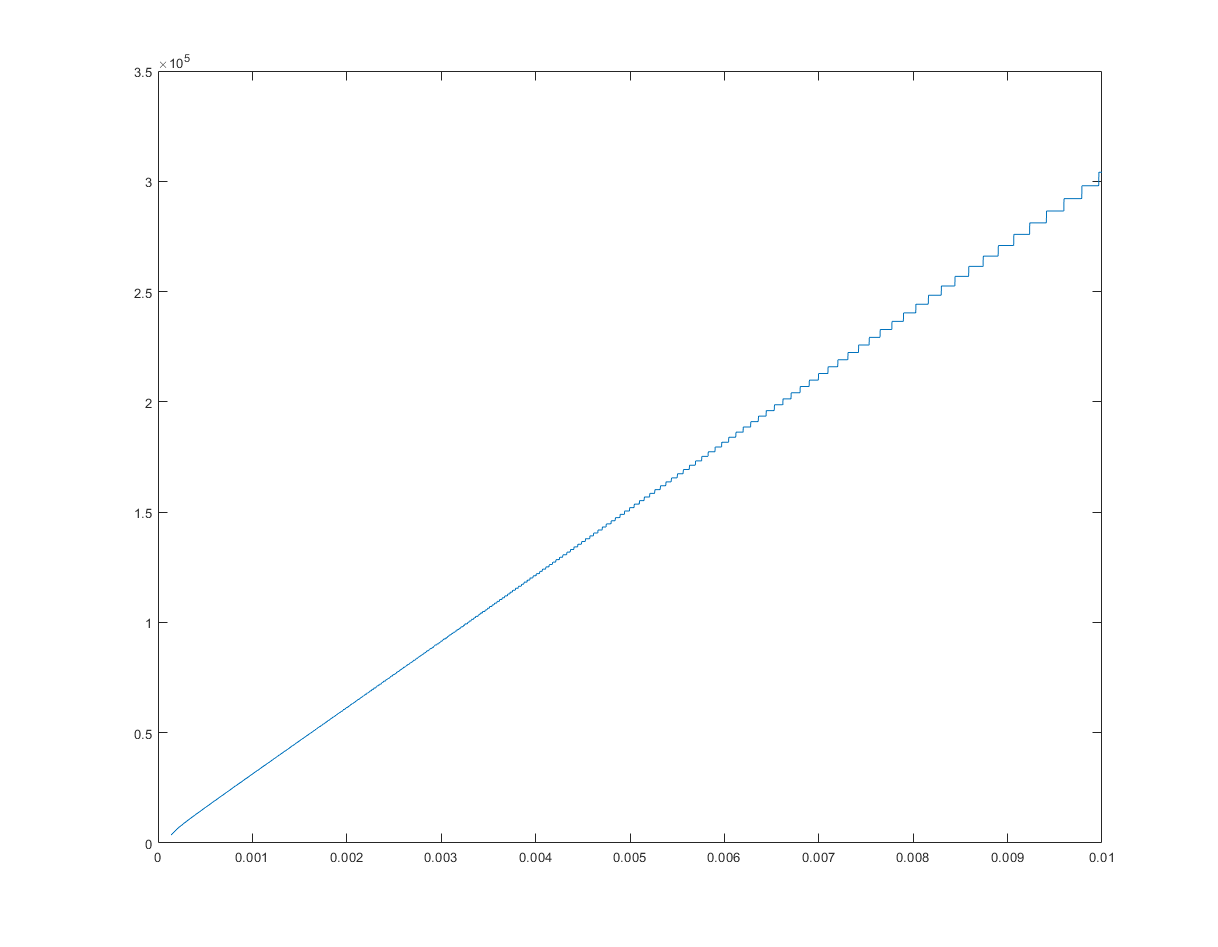
\includegraphics[width=1.1\textwidth]{ml-clk-freq-curve.png}}
		\caption[Curva frecuencia-tiempo del reloj de frecuencia variable]{Curva frecuencia-tiempo del reloj de frecuencia variable}
		\label{fig:ml-clk-freq-curve.png}
	\end{figure}

	Salvo errores de resolución por ser un dataset discreto y finito, la curva coincide con el resultado esperado. Queda demostrado que el reloj de frecuencia variable funciona, y las ecuaciones que describen su comportamiento son las expuestas en \ref{eq:clk-freq_eqs_freq}.
	
	Para las demás simulaciones se usarán scripts muy similares, ya que también estaremos analizando ondas cuadradas cuyo parámetro de interés es la frecuencia.	


	\subsection{Simulación del DAC por capacidades conmutadas}
	
	Este es el esquemático en LTSpice usado para simular el DAC por capacidades conmutadas:
	
	\begin{figure}[H]
		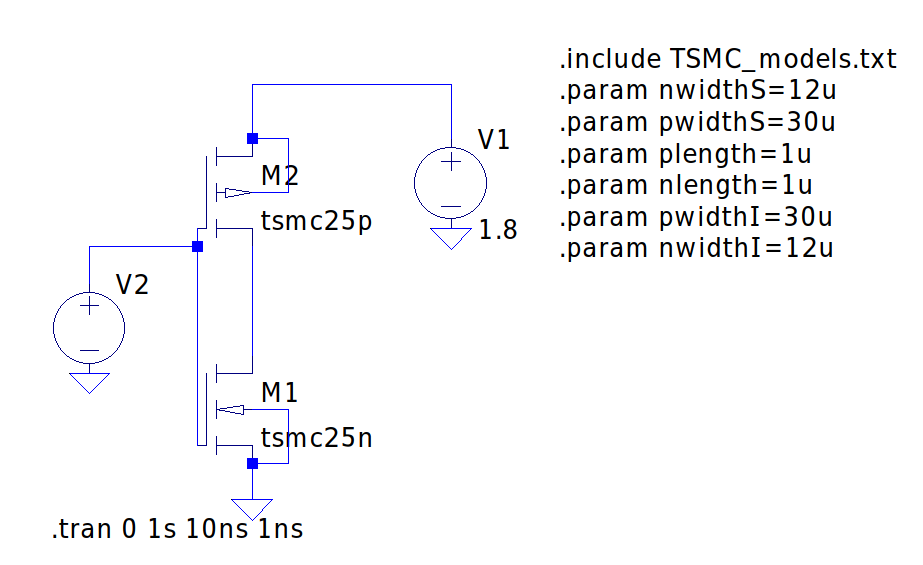
\includegraphics[width=0.8\textwidth]{ltspice-sw-cap-empty.png}
		\caption[Esquemático en LTSpice del modelo de DAC por capacidades conmutadas]{Esquemático en LTSpice del modelo de DAC por capacidades conmutadas}
		\label{fig:ltspice-sw-cap-empty.png}
	\end{figure}
	
	En la esquina superior derecha se reúnen los parámetros básicos de los transistores: sus dimensiones en ancho y largo. Los valores usados se corresponden con %TODO: por qué usamos estos tamaños de transistor para simular??
	%TODO: explicar por qué tienen tamaños diferentes??
	% TODO: explicar por qué no hay condensador!
	El voltaje de referencia escogido, 1.8V, %TODO: por qué 1.8??
	
	Añadimos el reloj de frecuencia variable explicado anteriormente:

	\begin{figure}[H]
		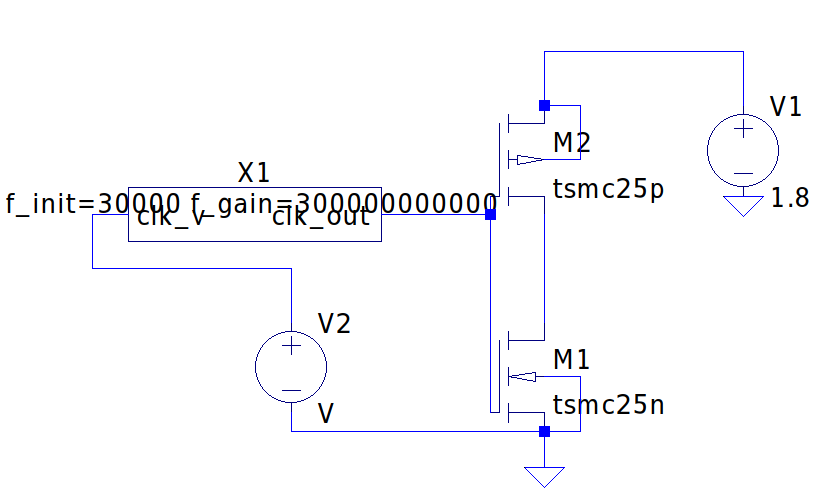
\includegraphics[width=0.8\textwidth]{ltspice-sw-with-clk-freq.png}
		\caption[Esquemático del circuito de capacidades conmutadas con reloj de frecuencia variable]{Esquemático del circuito de capacidades conmutadas con reloj de frecuencia variable}
		\label{fig:ltspice-sw-with-clk-freq.png}
	\end{figure}

	Como se puede observar en el esquemático, no se ha incluido un condensador en paralelo a la puerta. Esto es así porque los propios transistores tienen una capacitancia fruto de las corrientes parásitas. Esta capacitancia, presente en el modelo SPICE de los transistores que estamos usando, es del orden de unos 5 fF, suficiente para el correcto funcionamiento del DAC.

	Esta es la forma de onda resultante de la simulación:
	
	\begin{figure}[H]
		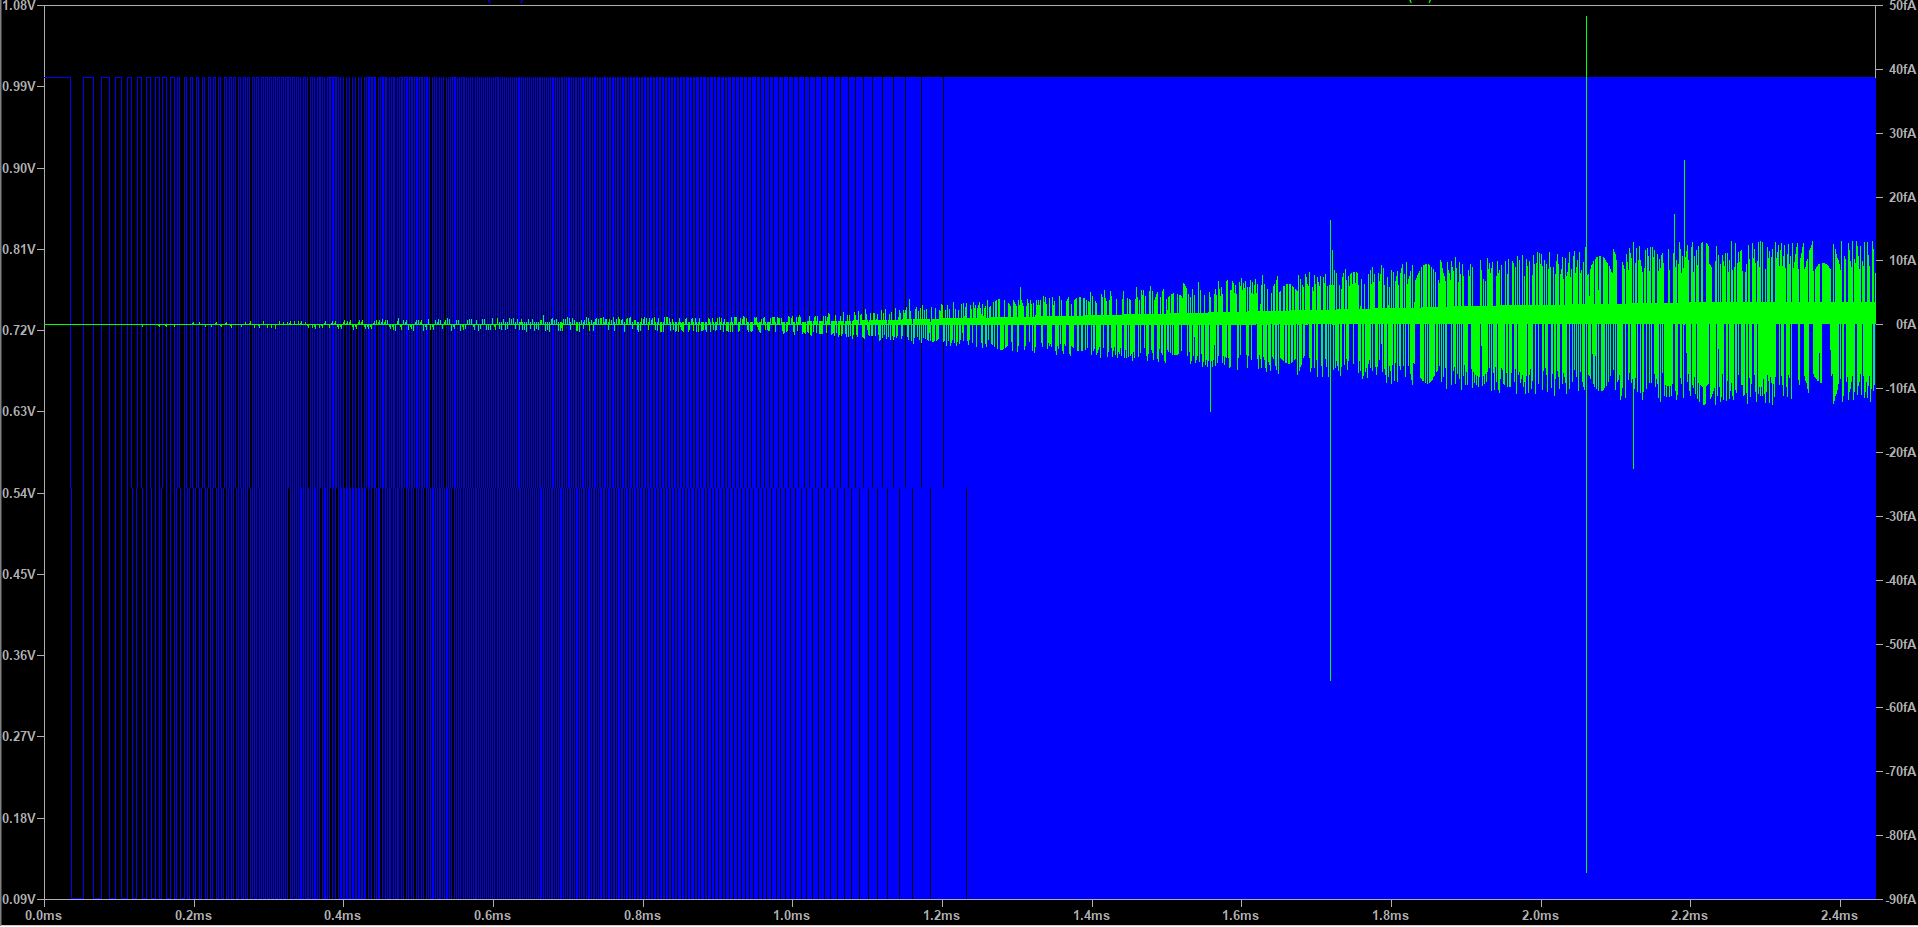
\includegraphics[width=0.8\textwidth]{dac-sim-waveform.png}
		\caption[Forma de onda de la simulación del DAC en el esquemático \ref{fig:ltspice-sw-with-clk-freq.png}]{Forma de onda de la simulación del DAC en el esquemático \ref{fig:ltspice-sw-with-clk-freq.png}}
		\label{fig:dac-graph-waveform.png}
	\end{figure}

	La señal azul corresponde al reloj de frecuencia variable, y la señal verde es la corriente que circula por el transitor inferior (canal-n) hacia tierra. Medimos en este punto porque en el lazo de realimentación del VCO conectaremos este nodo donde ahora está la tierra a la señal de entrada.
	
	Para obtener la curva de respuesta de este DAC, debemos analizar la forma de onda para relacionar la frecuencia del reloj con la corriente media. Usamos de nuevo el código del apartado \ref{lst:code-clk-var} para obtener los periodos de la señal del reloj. Para obtener la corriente media en cada periodo, haremos la media de los puntos del vector de corriente normalizado (uniformemente espaciado) entre cada uno de los puntos de comienzo de período.
	
\begin{lstlisting}[caption={Código en Matlab/Octave para el cálculo de la corriente media por cada periodo}, label={code-dac-i-mean}]
means = [];
for i = 1:(length(timestamp_periods))
	if i == 1
		means(i) = mean(dataset_eq_spaced(1:timestamp_periods(1,1), 2));
	else
		means(i) = mean(dataset_eq_spaced(timestamp_periods(i-1,1):timestamp_periods(i,1), 2));
	end
end
\end{lstlisting}

	Dibujamos la gráfica frecuencia-corriente media:
	
	\begin{figure}[H]
		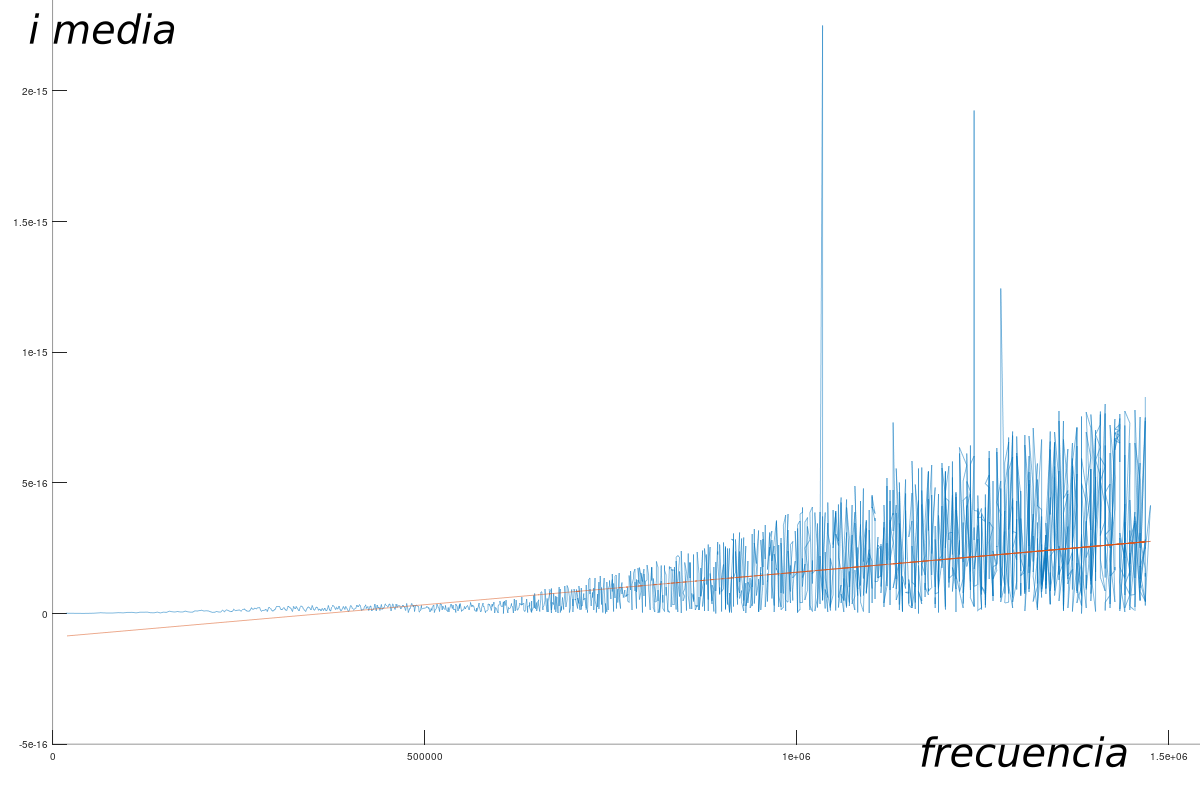
\includegraphics[width=1\textwidth]{dac-sim-graph.png}
		\caption[Gráfica frecuencia-corriente media para el DAC]{Gráfica frecuencia-corriente media para el DAC}
		\label{fig:dac-sim-graph.png}
	\end{figure}

	La gráfica azul representa la curva frecuencia-corriente media tal y como se ha procesado con el script expuesto más arriba. En rojo, se ha hecho una regresión lineal de dicha curva. Se puede observar una gran cantidad de ruido en la curva. Esto es así por varios motivos: los ciclos de carga y descarga del condensador (en este caso, capacitancia intrínseca de los transistores) no se simulan correctamente, apareciendo picos de descarga que no se corresponden con la realidad (observar los tres picos de la curva azul). Más allá de esto, la exactitud de la simulación viene de la mano del paso de simulación: a más frecuencia del reloj, menor paso de simulación se necesita para poder muestrear correctamente las señales de interés. Esto supone un problema por limitaciones de hardware: la simulación puede llegar rápidamente a ocupar decenas de gigabytes de memoria RAM, y otros tantos de disco. Las simulaciones expuestas en esta memoria se han llevado a cabo intentando explotar al máximo el hardware disponible para obtener la mayor exactitud posible, pero aún así ha sido inevitable la aparición de ruido como en la gráfica superior.
	
	En cualquier caso, se puede ver una tendencia creciente en las medias. A falta de una capacidad de simulación mejor, y respaldándonos en las ecuaciones \ref{sw-capacities-eqs}, asumiremos un comportamiento idealmente lineal del DAC por capacidades conmutadas de cara al desarrollo de los siguientes capítulos.
	
	%TODO: preguntar a Eric cómo queda esto
	
	\subsection{Modelo sencillo de ADC con VCO, abierto} %TODO: este título tampoco me gusta
	
	Partiendo del modelo \ref{fig:vco-adc-open-loop.png}, montamos el esquemático en LTSpice.
	
	\begin{figure}[H]
		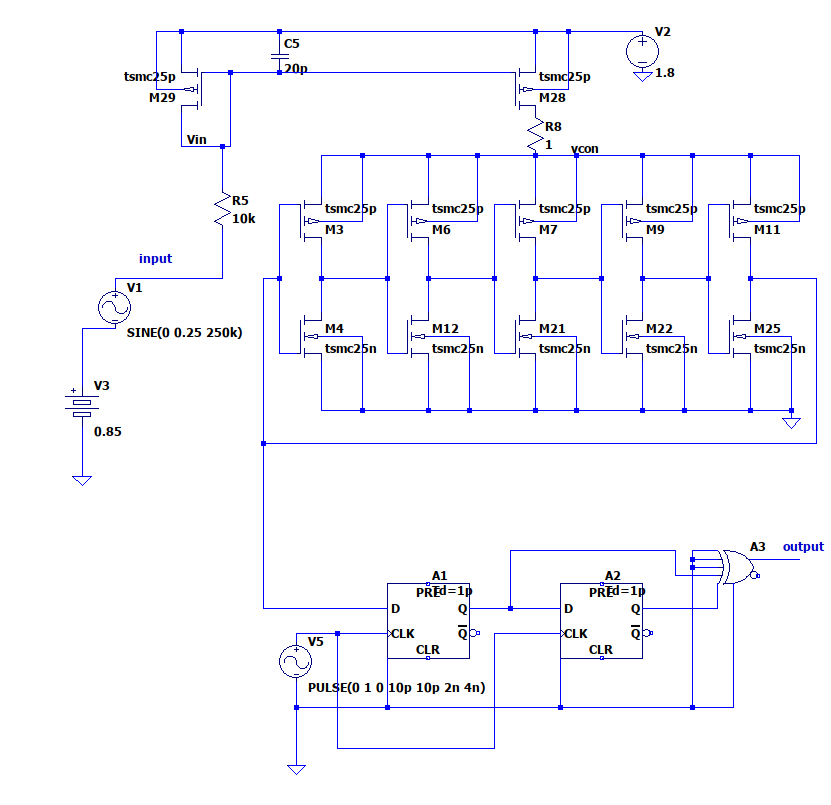
\includegraphics[width=\textwidth]{vco-open-first-diff-sch.png}
		\caption[Esquemático del ADC por VCO, abierto]{Esquemático del ADC por VCO, abierto}
		\label{fig:vco-open-first-diff-sch.png}
	\end{figure}
	
	A la izquierda tenemos un generador de señal sinusoidal de 250kHz con offset de 0.85V y amplitud 0.5V. Así se emula las características de las posibles señales a capturar en las aplicaciones a las que va destinado el sistema. En la parte superior, tenemos un espejo de corriente CMOS, que sirve para acoplar la señal de entrada a la entrada del VCO, actuando como buffer para evitar interacciones entre ambos bloques del sistema.
	En el centro está el VCO sencillo de cinco puertas, llamadas fases en el caso de un VCO. 
	
	
	Para demodular la señal del VCO (modulada en frecuencia), usamos un circuito de primera diferencia (en la parte inferior del esquemático, tomando la señal entre dos puertas cualquiera del VCO). Esta primera diferencia evalúa la diferencia entre dos señales de salida: una directa (primer flip-flop), y una retrasada un ciclo de reloj (segundo flip-flop). Ambas señales pasan por una puerta XOR para terminar de demodularse. El flujo de pulsos de 1 bit presente en la salida (output) equivale a los flancos de la señal del VCO, muestreados a la frecuencia del reloj conectado a los flip-flops. Así es como se demodula la señal que sale del VCO.
	
	%TODO: explicar esto mejor? añadir referencias?
	
	Este es el resultado de la simulación:
	
	\begin{figure}[H]
		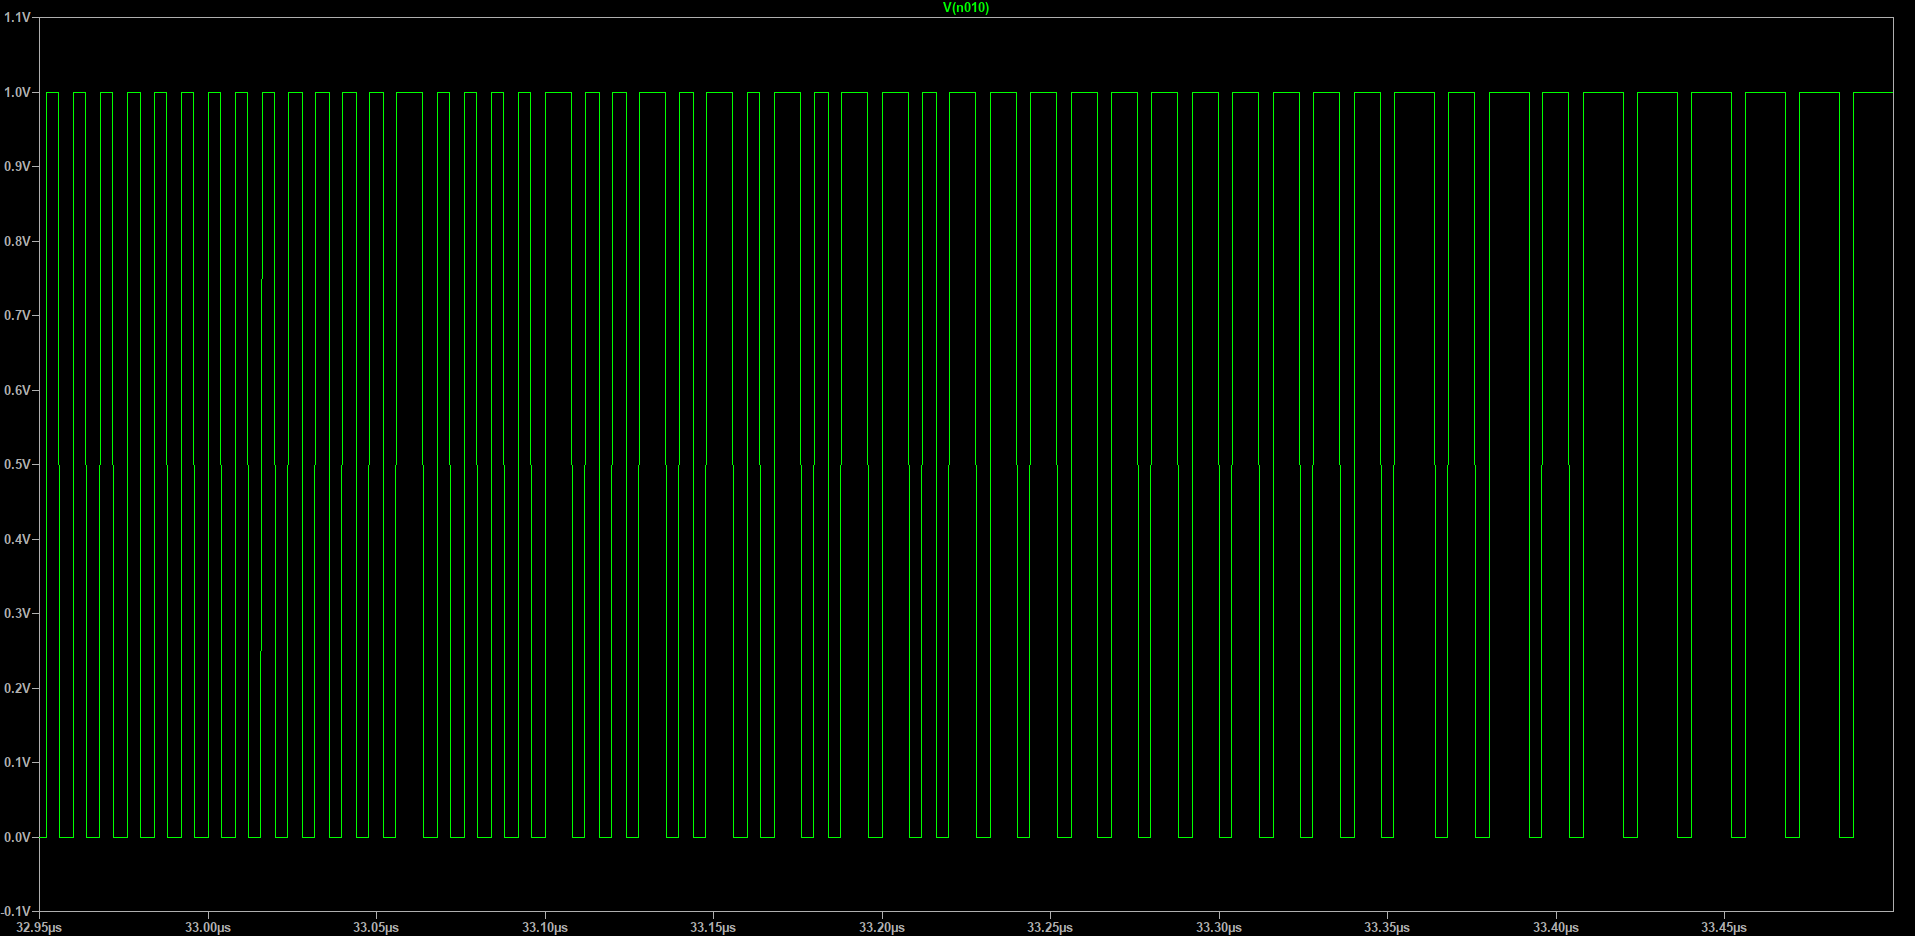
\includegraphics[width=\textwidth]{vco-open-first-diff-waveform.png}
		\caption[Detalle de la forma de onda de la simulación del VCO abierto]{Detalle de la forma de onda de la simulación del VCO abierto}
		\label{fig:vco-open-first-diff-waveform.png}
	\end{figure}

	Nótese que se ha escogido un rango cualquiera del total de la simulación, para poder apreciar mejor la forma de onda.
	
	Como se puede observar, la forma de onda en \ref{fig:vco-open-first-diff-waveform.png} es perfectamente cuadrada, ya que se ha sometido a la demodulación por la primera diferencia.
	
	Para analizar el comportamiento del sistema, usaremos la transformada rápida de Fourier. Compararemos el espectro de la señal original con el de la señal de salida ya demodulada.
	
	\begin{figure}[H]
		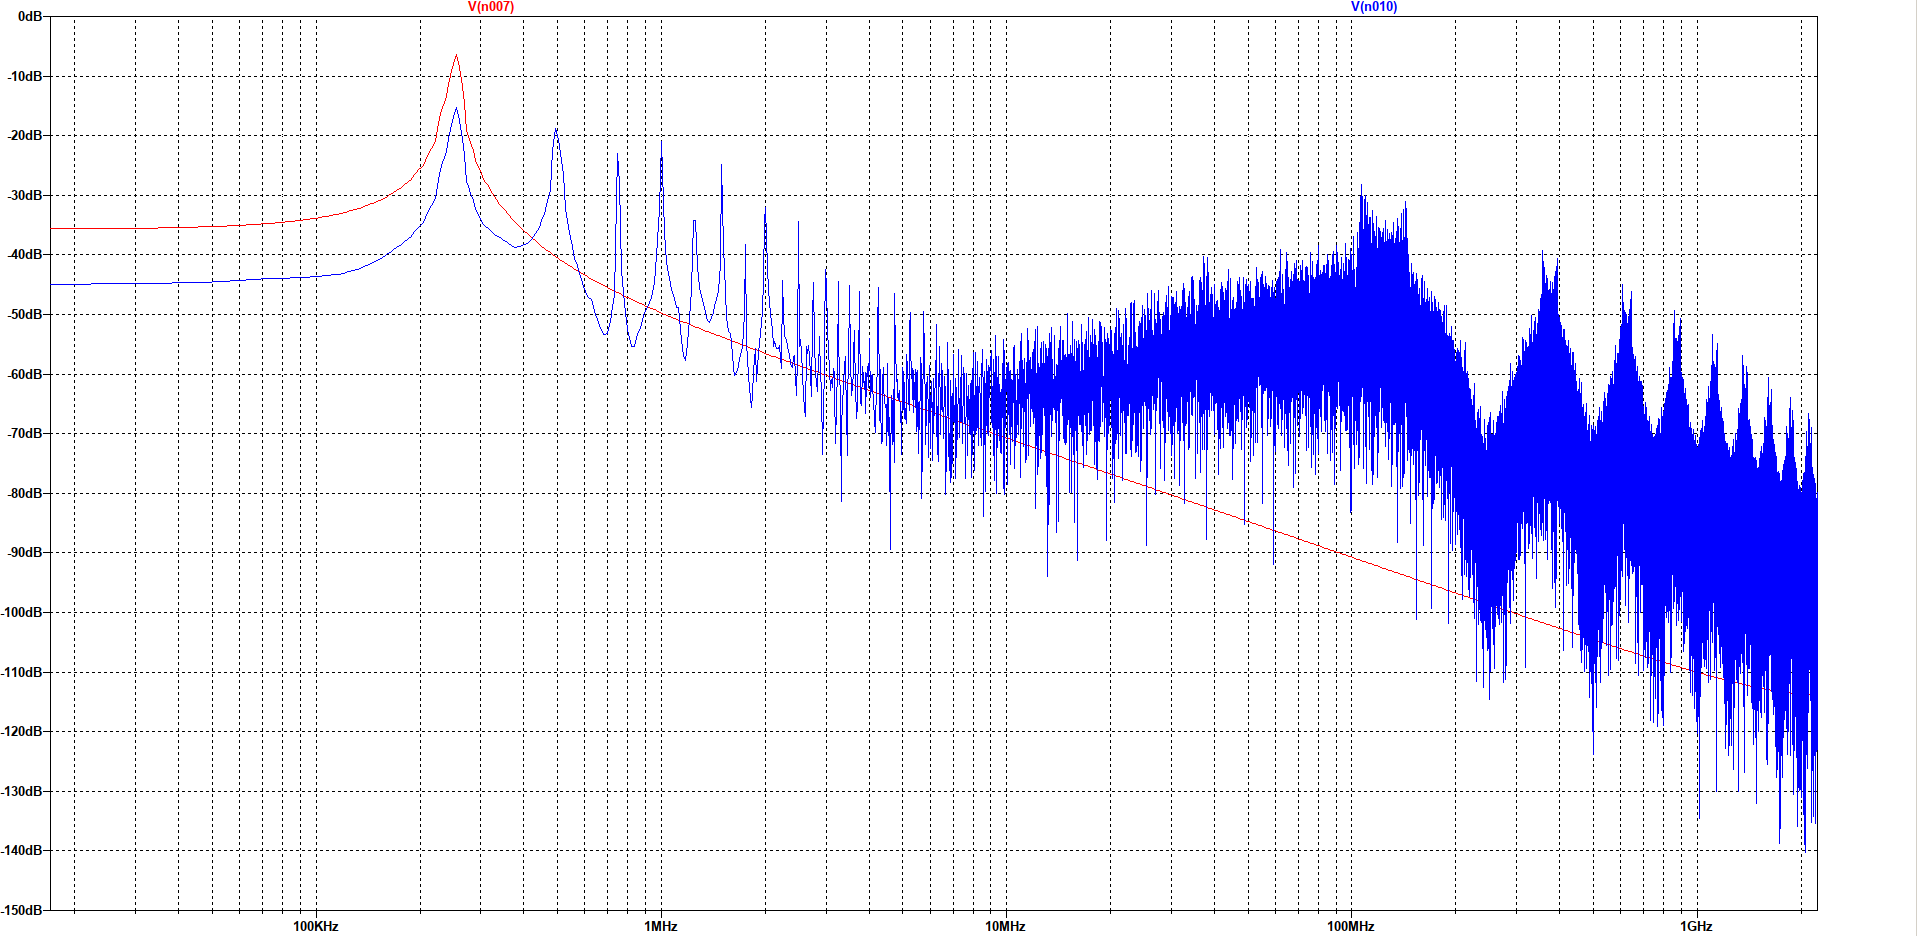
\includegraphics[width=\textwidth]{vco-open-first-diff-fft-2.png}
		\caption[FFT de la señal demodulada del VCO abierto]{FFT\footnote{Fast Fourier Transform, o transformada rápida de Fourier} de la señal demodulada del VCO abierto}
		\label{fig:vco-open-first-diff-fft-2.png}
	\end{figure}

	Para mejorar la visualización, se ha optado por un fondo blanco, con trazos de color rojo para la señal original y color azul para la señal de salida demodulada.
	
	En la FFT \ref{fig:vco-open-first-diff-fft-2.png} se puede ver que la señal original ha sido correctamente modulada y demodulada, porque el primer harmónico coincide con la frecuencia de la señal original, así como el segundo y tercero con sus múltiplos. El umbral de ruido es alto para frecuencias altas, pero limitando el ancho de banda esto no supone un problema. En los siguientes apartados trataremos de aumentar la ganancia del primer harmónico, disminuyendo la de los demás harmónicos y el umbral de ruido.
	
	\subsection{Modelo de ADC por VCO con bucle cerrado}\label{ss:vco-open}
	
	Visto el comportamiento de un VCO en bucle abierto, es el turno de probar cómo se comporta con un bucle de realimentación. Dado que el DAC no invierte la señal de entrada, debemos buscar una solución para hacer negativo el bucle de realimentación. La solución que hemos escogido para llevar esto a cabo es utilizar una estructura pseudodiferencial. Esto quiere decir que replicamos el circuito de VCO, lazo, y primera diferencia. Invertimos la señal de entrada en una de las ramas, para que ambos VCO trabajen con señales opuestas, y cruzamos los lazos de realimentación. Así conseguimos que que los lazos de realimentación actúen negativamente sobre sus respectivas entradas. % TODO: actúen negativamente???
	
	\begin{figure}[H]
		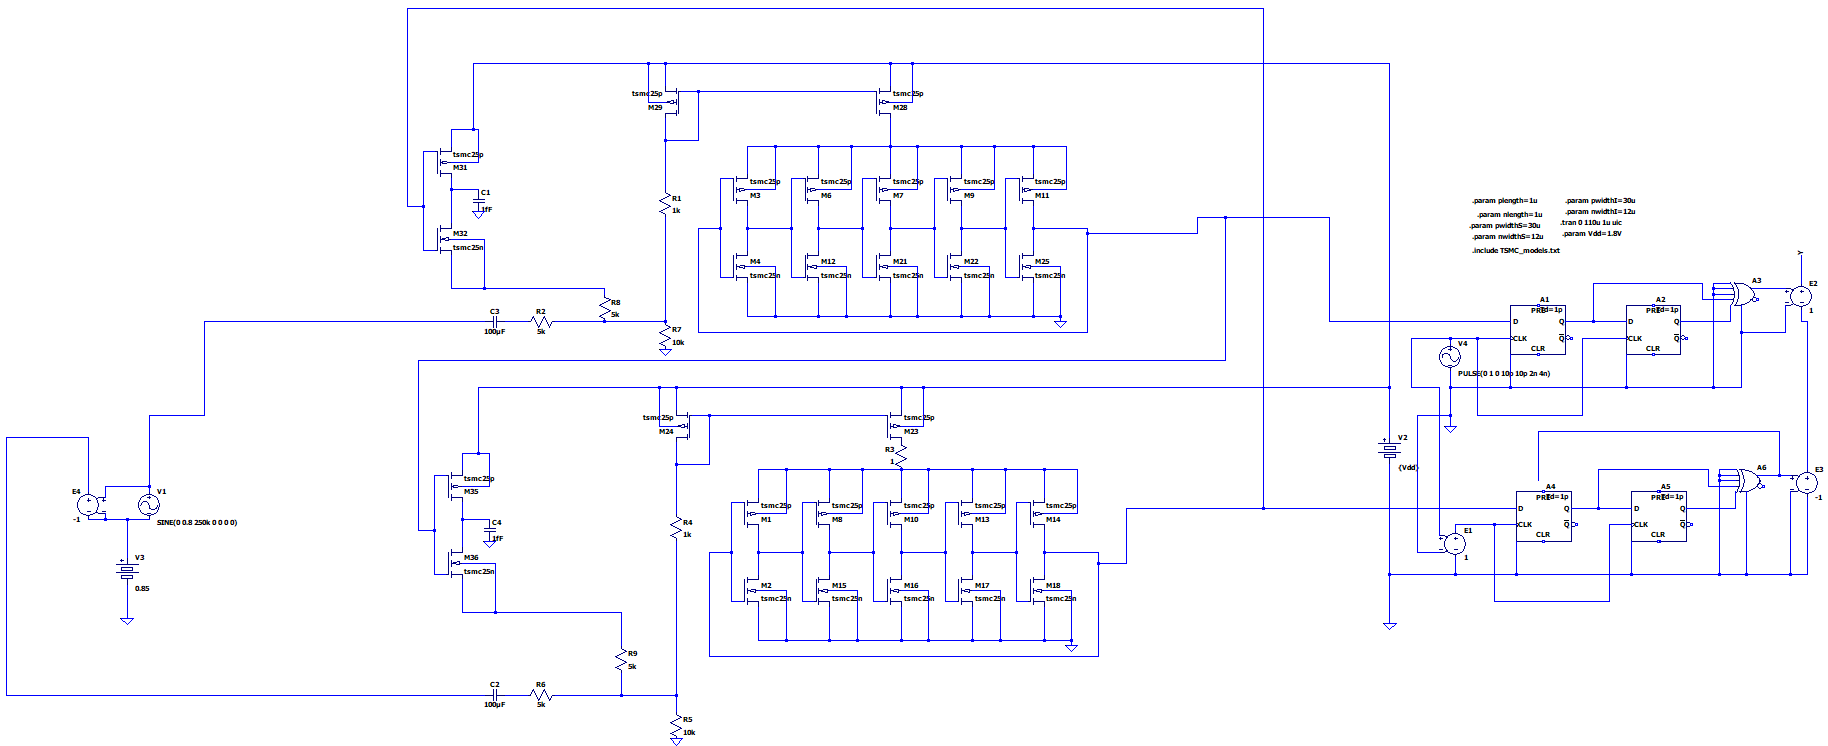
\includegraphics[width=\textwidth]{ltspice-vco-closed-diff.png}
		\caption[Esquemático del VCO con circuito de primera diferencia]{Esquemático del VCO con circuito de primera diferencia}
		\label{fig:ltspice-vco-closed-diff.png}
	\end{figure}

	% TODO: explicar todos los bloques!!!
	
	A continuación, se hará un análisis de cada bloque del circuito.
	
	Señal:
	
	\begin{figure}[H]
		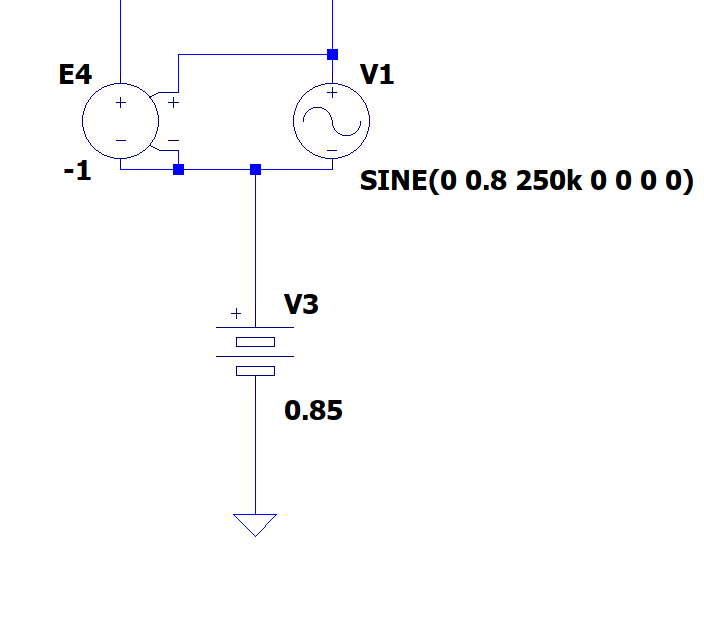
\includegraphics[width=0.6\textwidth]{ltspice-vco-closed-signal-block.png}
		\caption[Bloque de la señal del circuito de VCO con lazo cerrado]{Bloque de la señal del circuito de VCO con lazo cerrado}
		\label{fig:ltspice-vco-closed-signal-block.png}
	\end{figure}

	La señal de entrada del circuito es una señal sinusoidal de 250kHz de frecuencia y amplitud 0.8V con un offset de 0.85V. El offset está presente para evitar que aparezca voltaje negativo en el circuito, que entorpecería el funcionamiento del VCO y del resto de bloques del sistema. Para lograr la estructura pseudodiferencial, usamos un inversor de voltaje ($E4$) sobre la fuente de alterna $V1$. Cada una de las dos ramas superiores abastecerá a cada uno de los dos VCO.
	
	Realimentación y negador:
	
	\begin{figure}[H]
		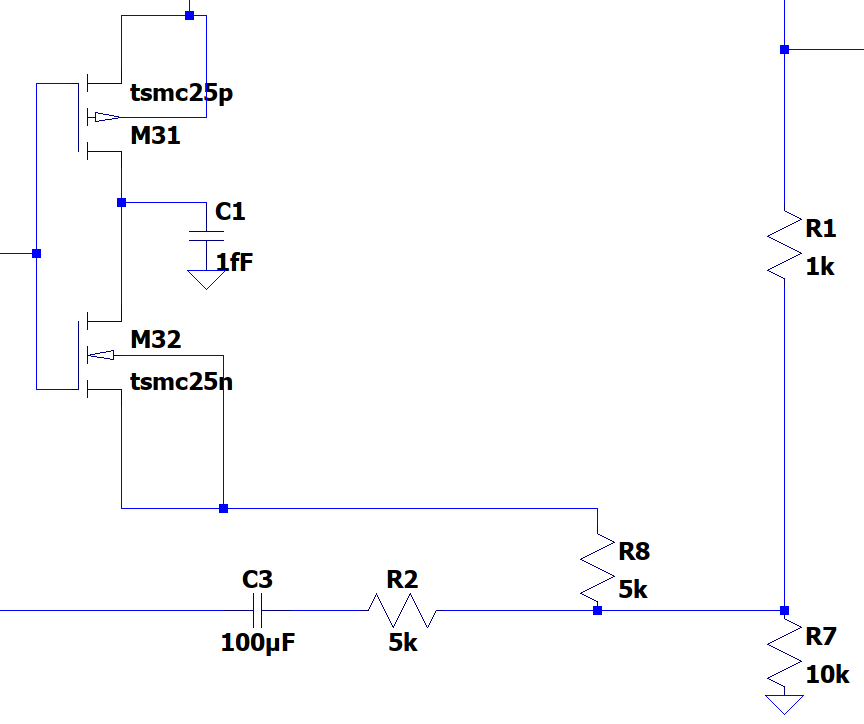
\includegraphics[width=\textwidth]{ltspice-vco-closed-loop-1.png}
		\caption[Bloque del lazo de realimentación y del negador del circuito de VCO con lazo cerrado]{Bloque del lazo de realimentación y del negador del circuito de VCO con lazo cerrado}
		\label{fig:ltspice-vco-closed-loop-1.png}
	\end{figure}

	El bloque anterior conecta con la rama inferior izquierda de este bloque. El condensador aparece para desacoplar la entrada del resto del circuito, y evitar interacciones no deseadas entre los componentes. Las resistencias forman un divisor de voltaje que compone el negador, aunque en principio se trate de un sumador entre la señal de entrada y la del lazo de realimentación de la rama opuesta de la estructura pseudodiferencial. El DAC por capacidades conmutadas aparece en la parte superior izquierda. La señal del DAC entra por su parte izquierda, y viene del VCO opuesto. La alimentación del DAC viene en su parte superior, de valor 1.8V, conectando con la fuente del transistor canal-p. El condensador entre los drenadores de los transistores es el encargado de lograr el efecto de la capacidad conmutada. La salida de este bloque al siguiente aparece en la esquina superior derecha, inmediatamente después del transistor de 1K.
	
	Entrada al VCO:
	
	\begin{figure}[H]
		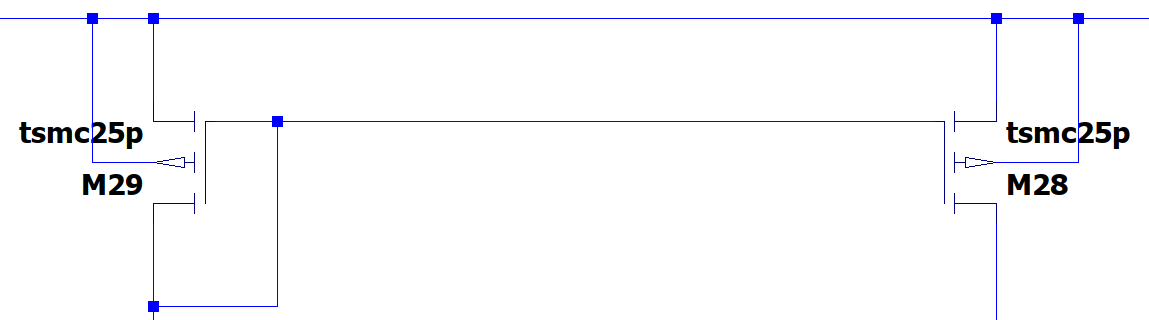
\includegraphics[width=\textwidth]{ltspice-vco-closed-current-mirror-block.png}
		\caption[Bloque de la entrada al VCO del circuito de VCO con lazo cerrado]{Bloque de la entrada al VCO del circuito de VCO con lazo cerrado}
		\label{fig:ltspice-vco-closed-current-mirror-block.png}
	\end{figure}

	Como buffer antes de la entrada al VCO, escogemos un espejo de corriente formado por dos transitores canal-p. Su función es replicar la corriente de entrada, en la esquina inferior izquierda, por la salida, en la esquina inferior derecha. La alimentación del espejo de corriente viene del rail superior, a un voltaje de alimentación común al sistema, igual al del DAC del bloque anterior, de 1.8V. Este buffer consigue separar la sección de entrada, compuesta por el bloque del negador y DAC de realimentación, del VCO. Así se evitan interacciones no deseadas entre componentes. %TODO: algo más???

	VCO:
		
	\begin{figure}[H]
		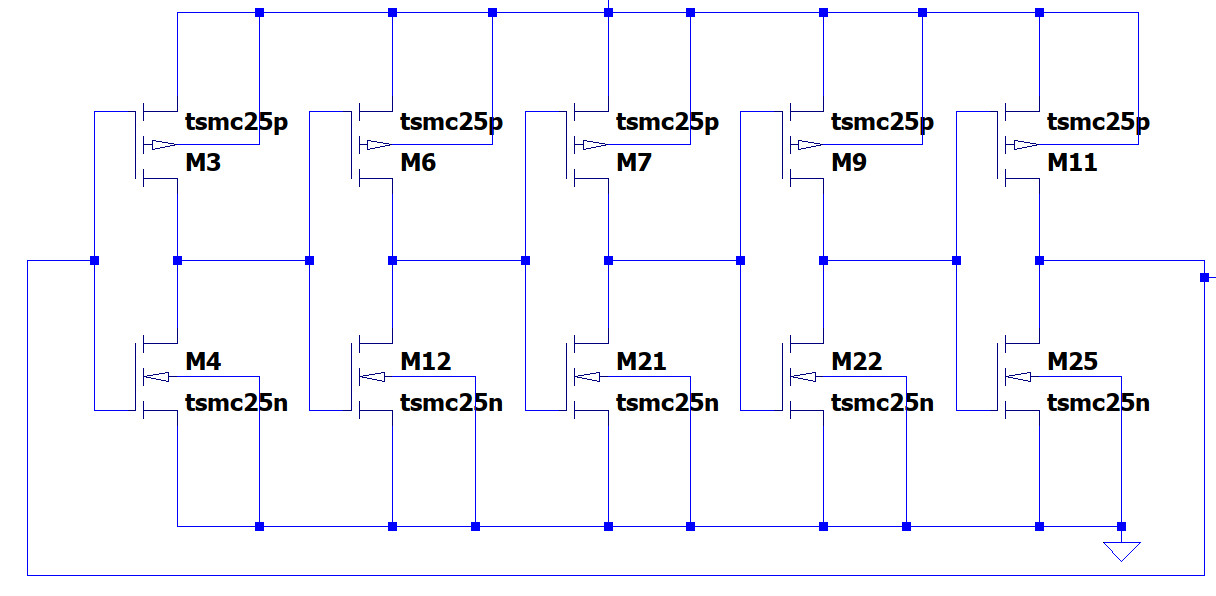
\includegraphics[width=\textwidth]{ltspice-vco-closed-vco-block.png}
		\caption[Bloque del VCO del circuito de VCO con lazo cerrado]{Bloque del VCO del circuito de VCO con lazo cerrado}
		\label{fig:ltspice-vco-closed-vco-block.png}
	\end{figure}

	Conectando con el espejo de corriente, tenemos el VCO. Este bloque ya se ha explicado en apartados anteriores. Tomamos el mismo número de fases que en el modelo de lazo abierto, es decir, cinco fases. La salida de este bloque está en su lado izquierdo, tomando la señal entre dos fases cualesquiera del VCO. Esta salida conecta con el circuito de primera diferencia, además de con el DAC del lazo de realimentación de la rama opuesta del sistema pseudodiferencial.

	Primera diferencia:
	
	\begin{figure}[H]
		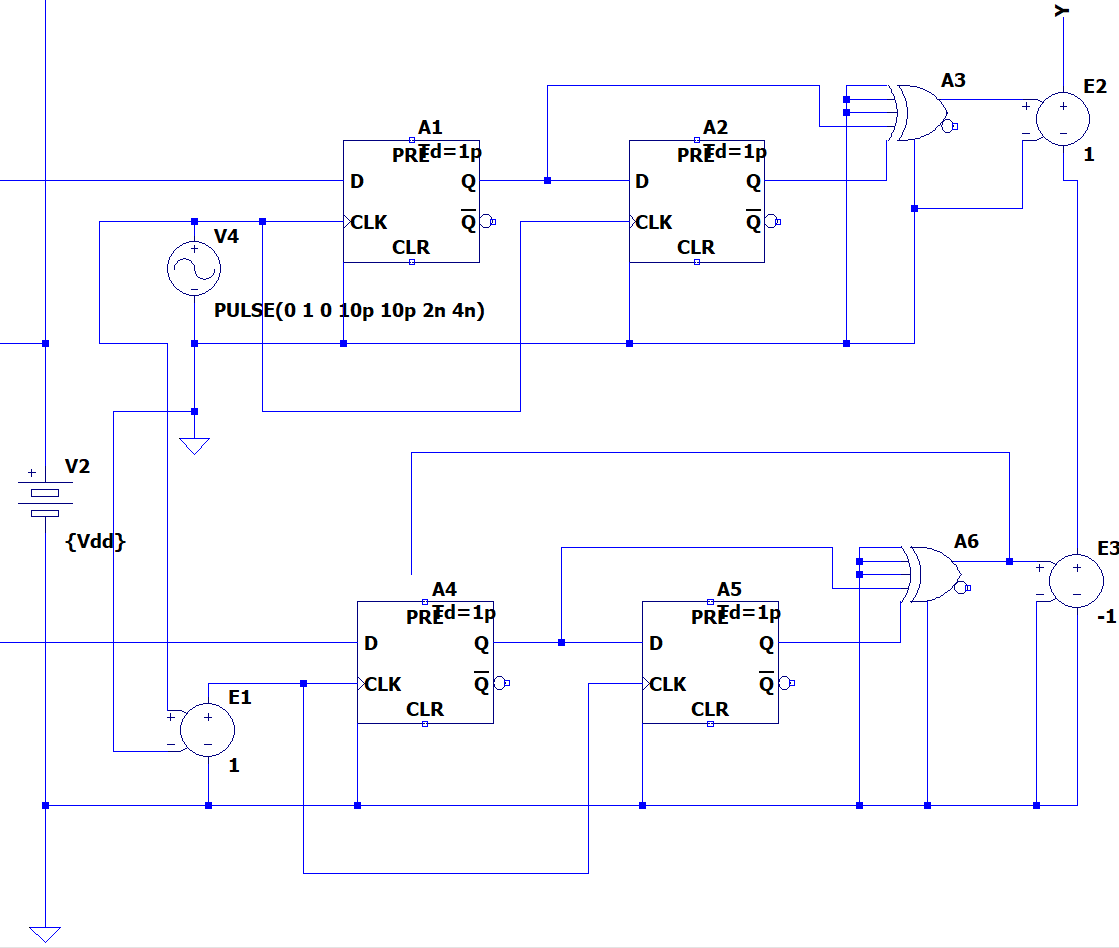
\includegraphics[width=\textwidth]{ltspice-vco-closed-diff-module.PNG}
		\caption[Bloque de la primera diferencia y salida del circuito de VCO con lazo cerrado]{Bloque de la primera diferencia y salida del circuito de VCO con lazo cerrado}
		\label{fig:ltspice-vco-closed-diff-module.PNG}
	\end{figure}

	Como en la sección anterior, \ref{ss:vco-open}, usamos un circuito de primera diferencia para demodular la señal del VCO. Como se observa en la imagen, y comparado con el circuito usado en el sistema con lazo abierto, \ref{fig:vco-open-first-diff-sch.png}, esta vez se duplican el número de componentes. Cada una de las ramas, conectada al pin $D$ de los flip-flops situados a la izquierda, necesita su propio demodulador, con su propio reloj. Como las ramas tienen como entradas señales de igual magnitud pero opuestas, los relojes también deben estar invertidos. El cambio más significativo con respecto al circuito \ref{fig:vco-open-first-diff-sch.png} es la inclusión de dos seguidores de tensión, $E1$ y $E2$, que se encargan de sumar las ramas, previa inversión de una de ellas, para compensar el desfase de la señal original. El resultado de todo el sistema aparece en la señal de salida $Y$, en la esquina superior izquierda. Es en este pin $Y$ donde mediremos los resultados en los siguientes apartados.
	
	Nótese también que en \ref{fig:ltspice-vco-closed-diff-module.PNG} aparece también la alimentación general del sistema, $V_{dd}$, que abaste al espejo de corriente y al DAC.
	
	
	Una vez explicados todos los elementos del sistema, procedemos a simular con los parámetros de entrada explicados en su correspondiente bloque.
	
	Este es el resultado de la simulación:
	
	\begin{figure}[H]
		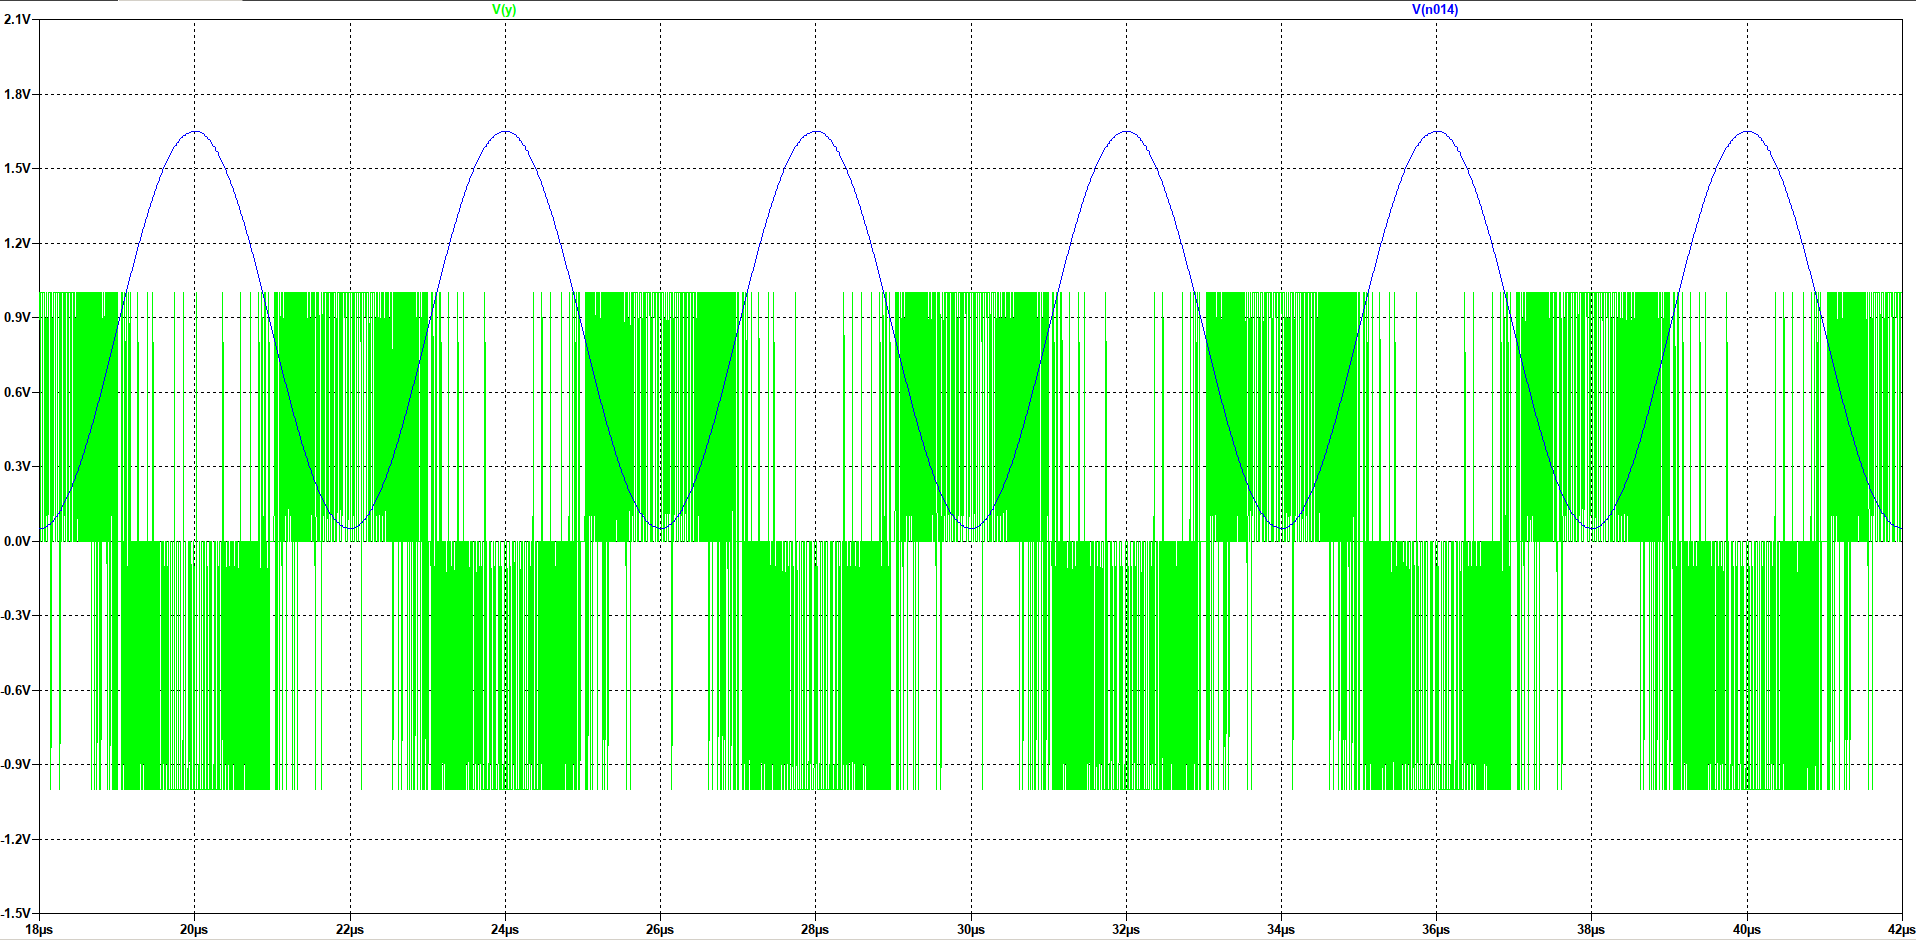
\includegraphics[width=\textwidth]{sim-vco-closed-waveform-dem.png}
		\caption[Forma de onda de la simulación del VCO con lazo de realimentación cruzado]{Forma de onda de la simulación del VCO con lazo de realimentación cruzado}
		\label{fig:sim-vco-closed-waveform-dem.png}
	\end{figure}

	En azul, tenemos la señal sinusoidal de entrada del sistema. En verde, la salida $Y$ final demodulada.
	
	Para apreciar mejor el detalle de la onda, ampliamos en una sección cualquiera.
	
	\begin{figure}[H]
		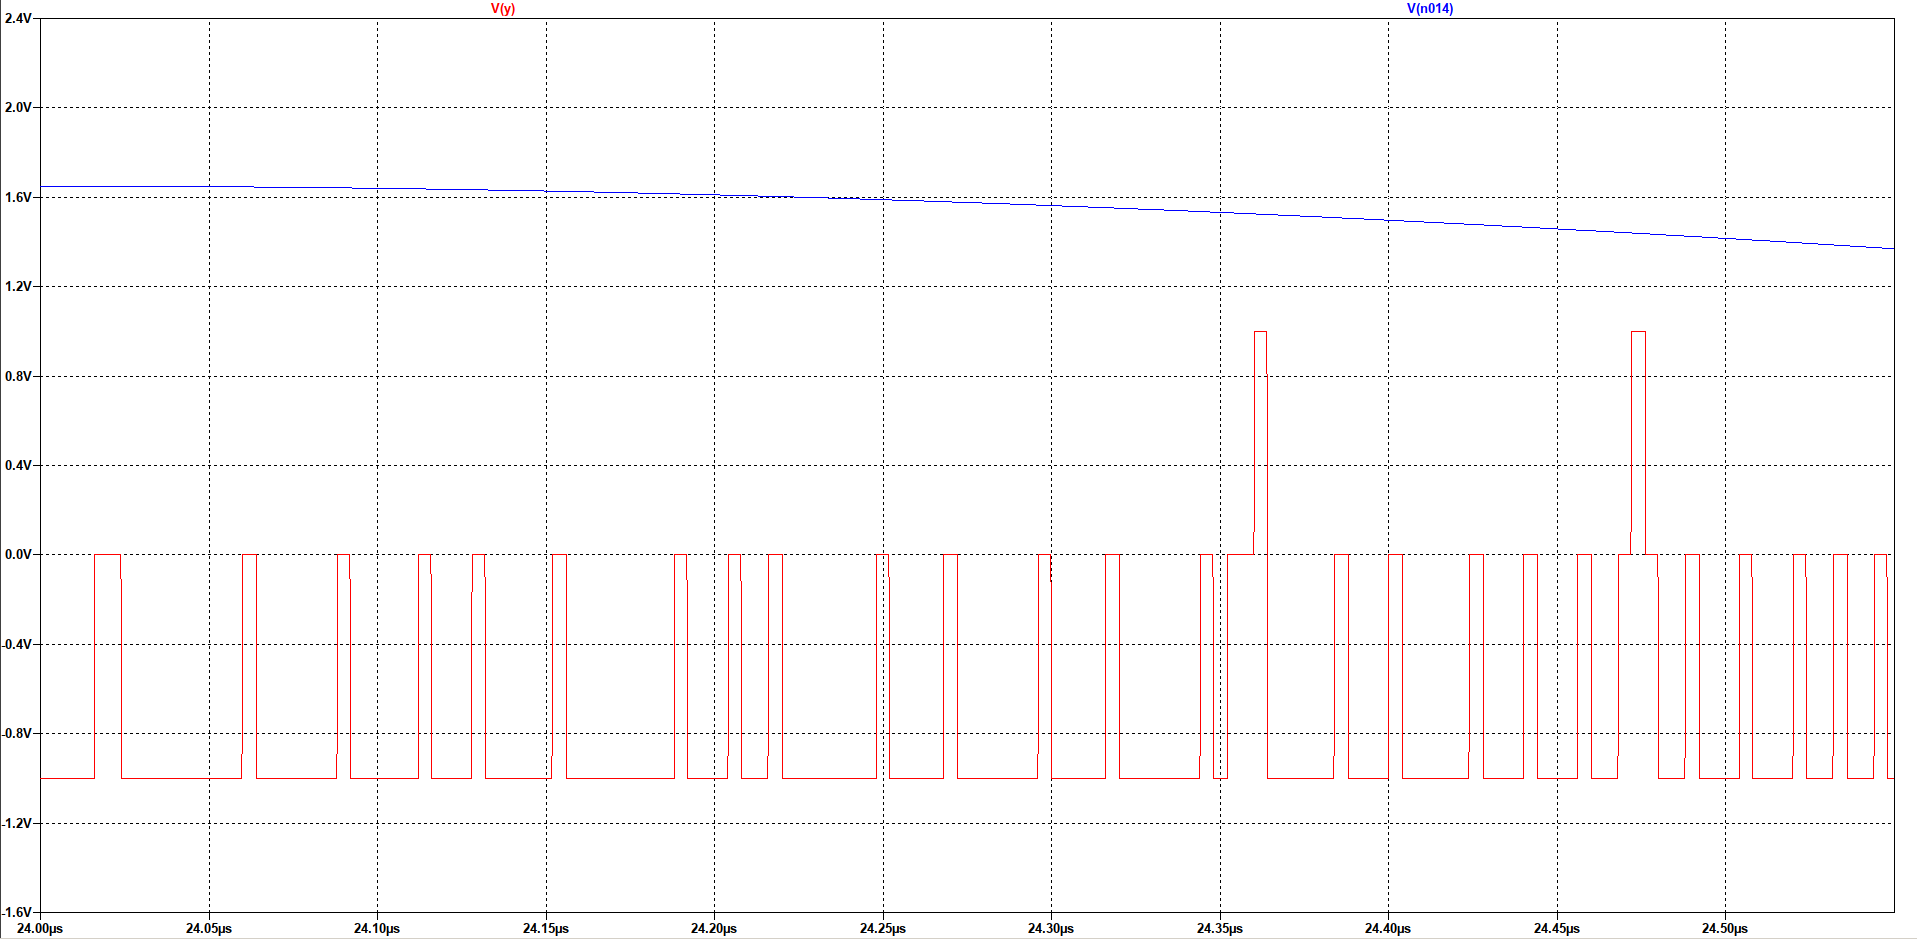
\includegraphics[width=\textwidth]{sim-vco-closed-waveform-dem-zoom.png}
		\caption[Detalle de la forma de onda \ref{fig:sim-vco-closed-waveform-dem.png}]{Detalle de la forma de onda \ref{fig:sim-vco-closed-waveform-dem.png}}
		\label{fig:sim-vco-closed-waveform-dem-zoom.png}
	\end{figure}

	Nótese que la señal de salida $Y$ se ha cambiado a color rojo para crear más contraste con el fondo y facilitar su lectura. La señal sinusoidal de entrada mantiene su color azul.

	 %TODO: comentario de esto. por qué queremos que haya dos señales inversas desfasadas 180 grados, una de ellas entre -1 y 0???
	
	El resultado de la modulación y demodulación de la señal se puede ver en la transformada rápida de Fourier:
	
	\begin{figure}[H]
		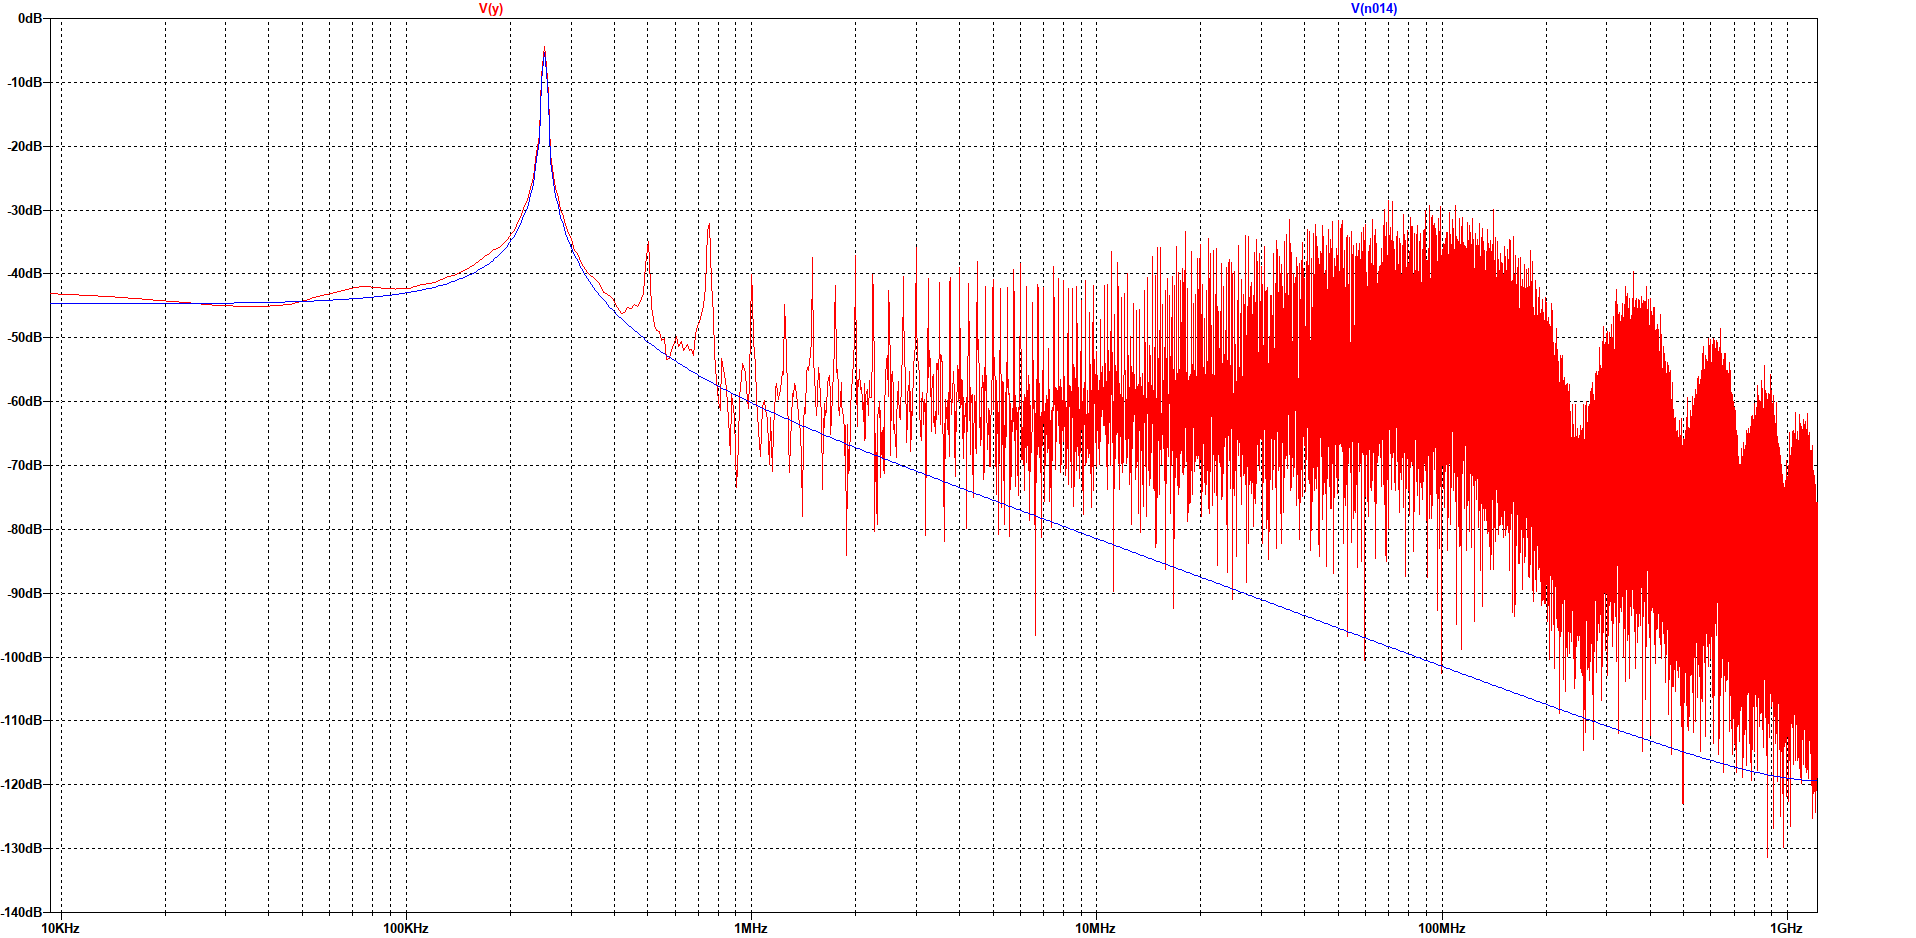
\includegraphics[width=\textwidth]{sim-vco-closed-waveform-dem-fft.png}
		\caption[FFT de la forma de onda \ref{fig:sim-vco-closed-waveform-dem.png}]{FFT de la forma de onda \ref{fig:sim-vco-closed-waveform-dem.png}}
		\label{fig:sim-vco-closed-waveform-dem-fft.png}
	\end{figure}
	
	En rojo, tenemos la señal final demodulada $Y$. En azul, tenemos la señal original que entra al sistema. Como se puede observar, hasta el harmónico principal la diferencia entre la señal original y la digitalizada es mínima. A partir de este primer pico, aparecen harmónicos secundarios, y apartir de 1MGHz, aparece una fuerte distorsión. Esta distorsión es fruto de todo el proceso de cuantificación. Corresponde al término $Q(s)$ %TODO: y $D(s)$ también???
	en las ecuaciones \ref{vco-closed-loop-s}.
	
	Comparando con la figura \ref{fig:vco-open-first-diff-fft-2.png}, la ganancia del harmónico principal es unos 10dB mayor, acercándose a la señal original. Disminuyen notablemente los harmónicos secundarios también. El umbral de ruido se mantiene a unos niveles similares.
	
	Teniendo en cuenta que el sistema con bucle cerrado funciona correctamente, y que sus prestaciones son superiores con respecto al sistema con bucle abierto, solo queda probar la linealidad de la respuesta del sistema con respecto a la entrada.
	
	\section{Estudio de la linealidad del ADC por VCO con lazo cerrado}
	
	\section{Soluciones alternativas}
	
	Como se comentó en el apartado \ref{sc:initial-idea}, en este estudio tratamos de prescindir de componentes complejos y costosos, en espacio y en consumo, como el amplificador operacional, aprovechando la ganancia intrínseca del VCO y del lazo de realimentación. Aunque la arquitectura propuesta en el apartado \ref{ss:vco-open} funciona correctamente y supone una importante mejora sobre el modelo de lazo abierto, el error de linealidad no llega a corregirse completamente. En este último apartado exploramos una alternativa plausible que aprovecha gran parte de la arquitectura propuesta, añadiendo ganancia extra en el lazo de realimentación. Esta ganancia, según las ecuaciones \ref{vco-closed-loop-s}, hará que disminuya la magnitud del error de linealidad y de cuantificación. Probando que este parámetro es decisivo en las prestaciones de la arquitectura, queda como trabajo futuro explorar opciones alternativas al amplificador operacional, como arquitecturas de VCO diferentes (más fases, ) %TODO: terminar de redactar esto: fases y vcos en paralelo? esto tiene un nombre; también buscar un convertidor de frecuencia a corriente que aporte más ganancia
	
	Incluimos el amplificador operacional en configuración no inversora (para mantener la estructura pseudodiferencial) en el bloque de realimentación, inmediatamente después del circuito de capacidad conmutada:
	
	\begin{figure}[H]
		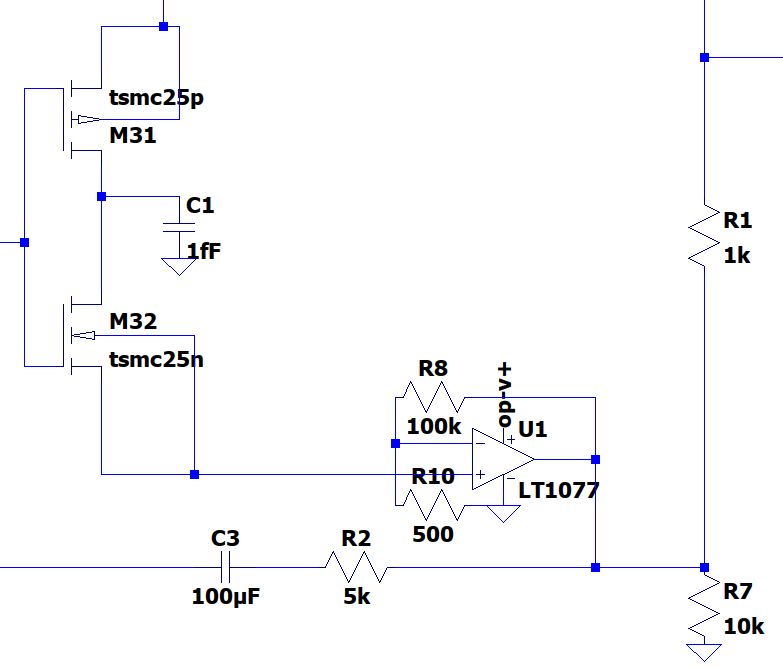
\includegraphics[width=\textwidth]{vco-closed-opamp-block.png}
		\caption[Bloque de alimentación modificado con amplificador operacional]{Bloque de alimentación modificado con amplificador operacional}
		\label{fig:vco-closed-opamp-block.png}
	\end{figure}
	
\chapter{Conclusiones (?)}
\chapter{Entorno socioeconómico (?)}
\chapter{Presupuesto / planificación / proceso (?)}

%----------
%	BIBLIOGRAFÍA
%----------	

\nocite{*} % Si quieres que aparezcan en la bibliografía todos los documentos que la componen (también los que no estén citados en el texto) descomenta está lína

\clearpage

\addcontentsline{toc}{chapter}{Bibliografía}

\setquotestyle[english]{british} % Cambiamos el tipo de cita porque en el estilo IEEE se usan las comillas inglesas.
\printbibliography

%----------
%	ANEXOS
%----------	

% Si tu trabajo incluye anexos, puedes descomentar las siguientes líneas
%\chapter* {Anexo x}
%\pagenumbering{gobble} % Las páginas de los anexos no se numeran



\end{document}